% Chapter 5

\chapter{Performance Study and Particle Identification}
\label{ch:PID} % For referencing the chapter elsewhere, use \autoref{ch:name}

%----------------------------------------------------------------------------------------

The goal of the present thesis being the extraction of identified hadrons, the RICH detector allows us to obtain the identity information from the hadron.
As the detector efficiency is not perfect, the misidentification probabilty is not zero ; one thus needs to determine the identification performance of the
RICH detector.
The RICH performance study relies on measuring the identification and misidentification probabilities for pions, kaons and protons. From samples of pure pions,
kaons and protons the RICH detector response is measured : the hadrons are identified using RICH informations and the identification and misidentification
probabilities are calculated in the hadron ($p_h$,$\theta_h$) phase space for pions, kaons and protons. The method used for identification is likelihood estimation
for different hypotheses. At first order, the mass assignment corresponds to the highest likelihood but further requirements can be added to improve the result.
The results obtained for the RICH performance are given in section \ref{sec:Results}.

\section{Determination of RICH Detector Performance}

The identification and misidentification efficiencies are given by the ration of the number of particles respectively correctly and wrongly identified out of pure
samples of known hadrons over the total number of hadrons composing the samples :

\begin{equation}
    P(t \rightarrow i) = \frac{N(t \rightarrow i)}{N(t)}
\end{equation}

$P(t \rightarrow i)$ is the probability that a hadron $t$ is identified as a hadron $i$, $N(t \rightarrow i)$ is the number of hadrons $t$ identified as $i$ and $N(t)$ is the total number of hadron $t$ of the pure sample. The identification ($P(t \rightarrow t)$) and misidentification ($P(t \rightarrow i)$) efficiencies are properties of the RICH and can be displayed in an efficiency matrix with the identification efficiencies are on the diagonal and the misidentification ones are off-diagonal.

\begin{equation}
  M_R
  =
  \begin{bmatrix}
  \epsilon(\pi \rightarrow \pi) & \epsilon(K \rightarrow \pi) & \epsilon(p \rightarrow \pi)\\
  \epsilon(\pi \rightarrow K) & \epsilon(K \rightarrow K) & \epsilon(p \rightarrow K) \\
  \epsilon(\pi \rightarrow p) & \epsilon(K \rightarrow p) & \epsilon(p \rightarrow p)
  \end{bmatrix}
\end{equation}

To obtain this matrix, three pure hadron samples are needed.

\subsection{Selection of $\Phi$, $K^0$ and $\Lambda$}

The RICH performance analysis is based on the study of the pion, kaon and proton samples coming from inclusive $\Phi$, $K^0$ and $\Lambda$.

In previous analysis on the RICH particle identification efficiency, exclusive $\Phi$ mesons were used. These are $\Phi$ meson produced in an exclusive reaction.
Therefore, only three particles are detected in the spectrometer. These are the scattered muon and the two kaons from the decay of the $\Phi$ meson. Such events do not represent typical events at COMPASS from deep inelastic scattering where also more than three particles are detected. Therefore, so called inclusive $\Phi$ mesons are used for the analysis. These are $\Phi$ mesons produced in deep inelastic scattering. Such events contain not only the scattered muon and the decay kaons from the $\Phi$ meson but might also contain additional particles. At high $z$, problems were found in the separation between kaons and pions using likelihood values\cite{}. This problem is not correctly taken into account using $K^0$ mesons. Therefore, a first test on using $\rho^0$ mesons instead is performed in order to determine the correct values for the identification and misidentification probabilities in this kinematic region.

For the determination of the RICH efficiency, it is necessary to have a source of events where the true kind of the particle passing the RICH is known. That kind of events is obtained using two body particle decays, namely the decay of a $K^0$ into two pions ($K^0 \rightarrow \pi^+\pi^-$), the $\Phi$ decay into two kaons ($\Phi \rightarrow K^+K^-$), the $\Lambda$ decay into a pion and a proton ($\Lambda \rightarrow p\pi^-$). In order to select such events with such decays, deep inelastic scattering events with a scattered muon are selected. The typical cuts are thus applied to the data:
\begin{itemize}
  \item Exclude bad spills
  \item Select best primary vertex with incoming and scattered muon
  \item Check if primary vertex is inside one of the target cells
  \item Extrapolated track of the incoming muon should cross all target cells
  \item $0.1 \le y \le 0.9$
\end{itemize}

Different selection criteria have to be used for $K^0$, $\Lambda$ and $\Phi$ decays. In the case of $K^0$ mesons and $\Lambda$ baryons, the particles decay by the weak force. Therefore, the decay length is long enough to produce a secondary vertex, which can be separated from the primary one. The $\Phi$ mesons decays by the strong force. This results in a very short decay length and it is not possible to separate the secondary vertex from the primary one.

\subsection{$K^0$ and $\Lambda$ selection}

For $K^0$ mesons the decay into $\pi^+$ and $\pi^-$ with a branching ration of (69.20 $\pm$ 0.05)\% \cite{} and in the case of $\Lambda$ and $\bar{\Lambda}$ baryons the decay into a proton and a pion with a branching ratio of (63.9 $\pm$ 0.5)\% \cite{} is used. In both decays the reconstruction of the secondary vertex is possible. The following cuts are applied to select these decays:

\begin{enumerate}
  \item Selection of good secondary vertices
  \begin{itemize}
    \item Loop over all vertices
    \item Vertex is not primary one
    \item Exactly two opposite charged outgoing particles
    \item The tracks should not be connected to any other primary vertex
    \item Primary and secondary vertex separated by more than 2$\sigma$
  \end{itemize}
  \item Select good hadron tracks
  \begin{itemize}
    \item Both particles should not have crossed more than 10 radiation length
    \item Last measured position ($Z_{last}$) behind SM1
    \item Transverse momentum with respect to the mother particle larger than 23 MeV to suppress electrons
    \item Check that the decaying particle is connected to the primary vertex ($\theta \le 0.01$)
  \end{itemize}
  \item Additional cuts
  \begin{itemize}
    \item $p_h \geq 1 GeV/c$
    \item Mass difference smaller than 150 MeV/c$^2$ between the $K^0$/$\Lambda$ mass and the invariant mass of the two decay hadrons assuming the correct masses
  \end{itemize}
\end{enumerate}

The same cuts except for the mass cuts are used for $K^0$ and $\Lambda$ candidates. For the selected candidates, the RICH likelihoods of the two decay particles are stored for further analysis. During the first selection step, good secondary vertices are selected with only two outgoing tracks. In order to ensure that the two tracks belong to this secondary vertex, the vertex is skipped if a track is assumed to originate from a primary vertex. In addition, the primary and secondary vertex should be separated from one another. Therefore, the distance between both should be larger than two times the reconstruction accuracy.
During the second selection step, good hadron tracks are selected. In order to suppress tracks from muons, tracks which have passed a large amount of material are rejected. In addition, only tracks with a measured momentum are selected. This is ensured by a last measured position behind the first spectrometer magnet. In addition, it is ensured that the $K^0$ meson and $\Lambda$ baryon is produced in the primary vertex by comparing the angle $\theta$ between their momentum vector and the vector connecting the primary and secondary vertex. Tracks from electrons are suppressed by removing particles with low transverse momenta with respect to the mother particle. This is shown in Fig. \ref{pic:Armenteros}. Here, the transverse momentum of a particle is shown as a function of the ratio of the longitudinal momentum ratio of two particles:

\begin{equation}
  \alpha = \frac{p_{L,1}-p_{L,2}}{p_{L,1}+p_{L,2}}
\end{equation}

\begin{figure}[!h]
  \centering
	% 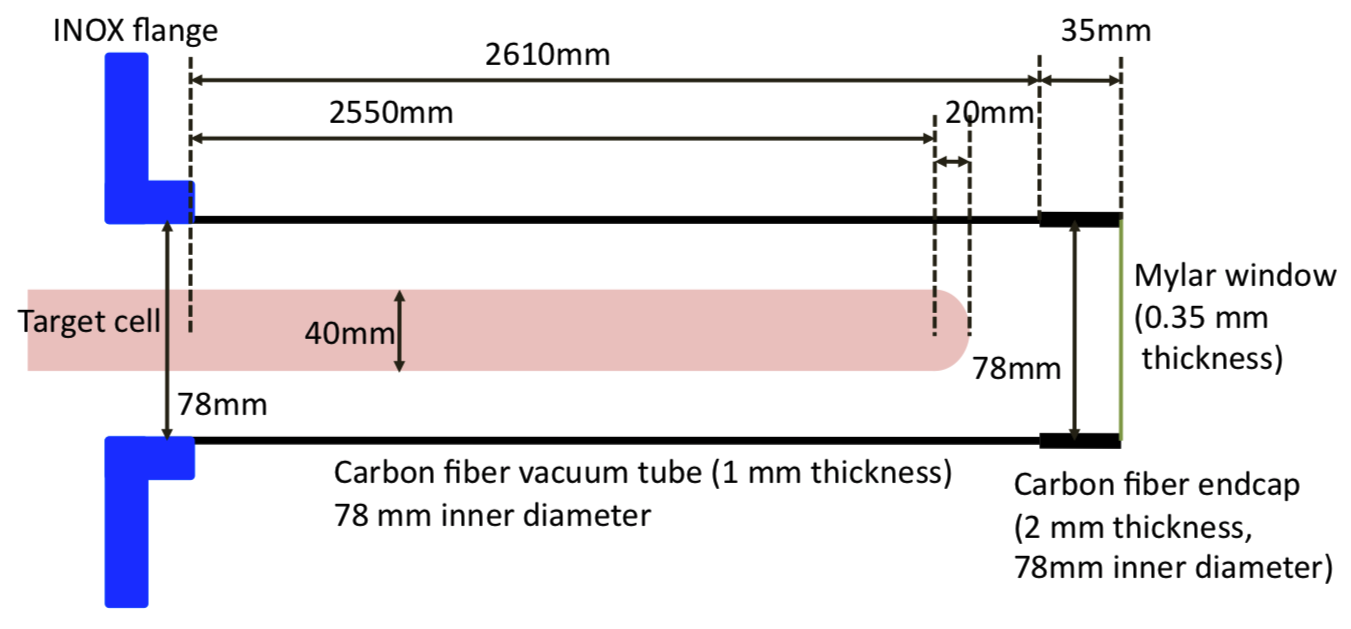
\includegraphics[scale=0.3]{./gfx/Target.png}
	\caption{Armenteros plot showing the effect of the cut on the transverse momemtum illustrated by the red line.}
	\label{pic:Armenteros}
\end{figure}

The three visible arcs are produced by the decay of the $K^0$ mesons and the $\Lambda$ baryons. The decay of $K^0$ mesons in two particles with the same mass results in the symmetric arc, whereas the decay of $\Lambda$ baryons into two particles with different masses result in the two smaller arcs on the left and right side. The band at the bottom is produced by electrons from pair production. These are removed by the cut on the transverse momentum. This is also shown in Figure 2 for the transverse momentum of the particles from decays of $K^0$ meson or $\Lambda$ baryon candidates.

During the third selection step, events, which will not be used in the later analysis, are removed. Therefore, a minimal momentum of the particle is required and only a mass range of 150 MeV/c2 around the $K^0$ or $\Lambda$ mass is selected. The effect of the cuts on the invariant mass of the $K^0$ and $\Lambda$ candidates is shown in Figure 3 in the range of their mass. The strongest reduction is achieved by requiring the production of the $K^0$ meson or $\Lambda$ baryons at the primary vertex.
In addition, also the effect of the Likelihood cuts for the particle identification, which are applied later one, is shown.

\subsection{$\Phi selection$}

The $\Phi$ meson decay length is too short to separate the primary and decay vertex. Therefore, all outgoing particles from a primary vertex are taken into account for the search of possible $\Phi$ mesons. The branching ratio of the decay into two kaons is (48.9 $\pm$ 0.5\%) \cite{}.

\begin{enumerate}
  \item Selection of possible good events with $\Phi$ mesons
  \begin{itemize}
    \item At least 3 outgoing particles including scattered muon
    \item Loop over all outgoing particles
    \item Oppositely charged pairs of hadrons (none is a muon)
  \end{itemize}
  \item Select good hadron tracks
  \begin{itemize}
    \item Last measured position ($Z_{last}$) behind SM1
    \item Transverse momentum with respect to the mother particle larger than 23 MeV to suppress electrons
  \end{itemize}
  \item Additional cuts
  \begin{itemize}
    \item 9 GeV/c $\leq p_h \leq$ 55 GeV/c
    \item Mass difference smaller than 120 MeV/c$^2$ between the $\Phi$ mass and the invariant mass of the two decay hadrons assuming the kaon masse.
  \end{itemize}
\end{enumerate}

The selection steps are similar the selection of the $K^0$/$\Lambda$ candidates. In the first step, primary vertices with oppositely charged hadron pairs are selected. During the second selection step, only particles with a measured momentum are kept and possible electrons are removed by removing particles with a too low transverse momentum. During the third step additional cuts are applied to remove events, which will not be used in the later analysis. The effect of the various cuts is shown in Figure 4. The selection of $\Phi$ meson candidates results in a large combinatorial background. During the selection the largest suppression is achieved by the removal of electrons. By also applying the Likelihood cuts to identify the kaons a large suppression can be achieved.

\section{RICH Particle Identification}

The goal of the selection is a clean pion and kaon sample. Due to the larger amount of pions compared to kaons stricter selection cuts are imposed for kaons. The identification of these particles is done using likelihood cuts. Using the likelihood values, the particle identification is done by comparing these values with one another. In the simplest case, the highest one determines the particle type. This method is used in the case of pions. In the case of kaons, stricter likelihood cuts are applied to suppress misidentified pions. These stricter cuts are an improvement compared to previous COMPASS analysis and are used in the multiplicity analysis. The likelihood cuts are listed in Table \ref{LHcut}. Also less stricter likelihood cuts are used, which are listed in Table \ref{LHlessstrict}. Similar cuts were used in the analysis of the hadron multiplicities using 2006 data. A further improvement is the inclusion of protons in the RICH particle identification efficiency determination. The RICH particle identification efficiency is studied in the momentum range of 10 GeV/c $ \leq p \leq $ 50 GeV/c. In this range, pions and kaons are emitting Cherenkov light, while up to $\sim$ 17 GeV protons are still below the threshold of

\begin{equation}
  p_{thr,i} = \frac{m_i}{ \sqrt{n^{2}-1} }
\end{equation}

where $n$ is the refractive index. This is shown in Fig. \ref{pic:RefIndex} where the reconstructed Cherenkov angle is shown as a function of the hadron momentum. As the momentum range is restricted to momenta larger than 10 GeV/c, no electron rejection can be performed. In this momentum range the Cherenkov angle for pions and electrons are too close to one another. Muons can also be not rejected using likelihood cuts as the Cherenkov angle for muon and pion is too close to one another. But they are identified using cuts on the radiation length passed by a particle. The identification of pions, kaons and protons above the momentum threshold is done by comparing the likelihood values with one another. The likelihood cuts for protons require its likelihood to be the largest one. These cuts are also given in Table. \ref{tab:LHcut}. Below the momentum threshold, protons do not emit Cherenkov light. Therefore, the likelihood values are used to test whether the detected light is consistent with random noise in the detector (background). In order to avoid possible problems due to the uncertainty on the reconstructed momentum or the uncertainty of the refractive index of the RICH gas, a region of $\pm$5 GeV/c around the proton threshold is used, where both hypothesis are applied for proton identification.

\begin{table}[!h]
  \caption{Likelihood cuts for pion, kaon and protons}
  \label{tab:LHcut}
  \centering
  \begin{tabular}{lcccc}
    \hline
     & PION & KAON & \multicolumn{2}{c}{PROTON} \\
    \hline
    MOMENTUM & $p$ > $p_{\pi,thr}$ & $p$ > $p_{K,thr}$ & $p$ $\leq$ $p_{p,thr}$ & $p$ > $p_{p,thr}$ \\
    Likelihood type \textit{i} & $\pi$ & $K$ & bg & $p$ \\
    LH(\textit{i})/LH($\pi$) & --- & > 1.08 & > 1.0 & > 1.0 \\
    LH(\textit{i})/LH(K) & > 1.0 & --- & > 1.0 & > 1.0 \\
    LH(\textit{i})/LH($p$) & > 1.0 & > 1.0 & --- & --- \\
    LH(\textit{i})/LH(bg) & > 1.0 & > 1.24 & --- & > 1.0 \\
    \hline
  \end{tabular}
\end{table}

\begin{table}[!h]
  \caption{Less strict likelihood cuts for pion, kaon and protons}
  \label{tab:LHlessstrict}
  \centering
  \begin{tabular}{lcccc}
    \hline
     & PION & KAON & \multicolumn{2}{c}{PROTON} \\
    \hline
    MOMENTUM & $p$ > $p_{\pi,thr}$ & $p$ > $p_{K,thr}$ & $p$ $\leq$ $p_{p,thr}$ & $p$ > $p_{p,thr}$ \\
    Likelihood type \textit{i} & $\pi$ & $K$ & bg & $p$ \\
    LH(\textit{i})/LH($\pi$) & --- & > 1.0 & > 1.0 & > 1.0 \\
    LH(\textit{i})/LH(K) & > 1.0 & --- & > 1.0 & > 1.0 \\
    LH(\textit{i})/LH($p$) & > 1.0 & > 1.0 & --- & --- \\
    LH(\textit{i})/LH(bg) & > 1.0 & > 1.07 & --- & > 1.0 \\
    \hline
  \end{tabular}
\end{table}

\begin{figure}[!h]
  \centering
	% 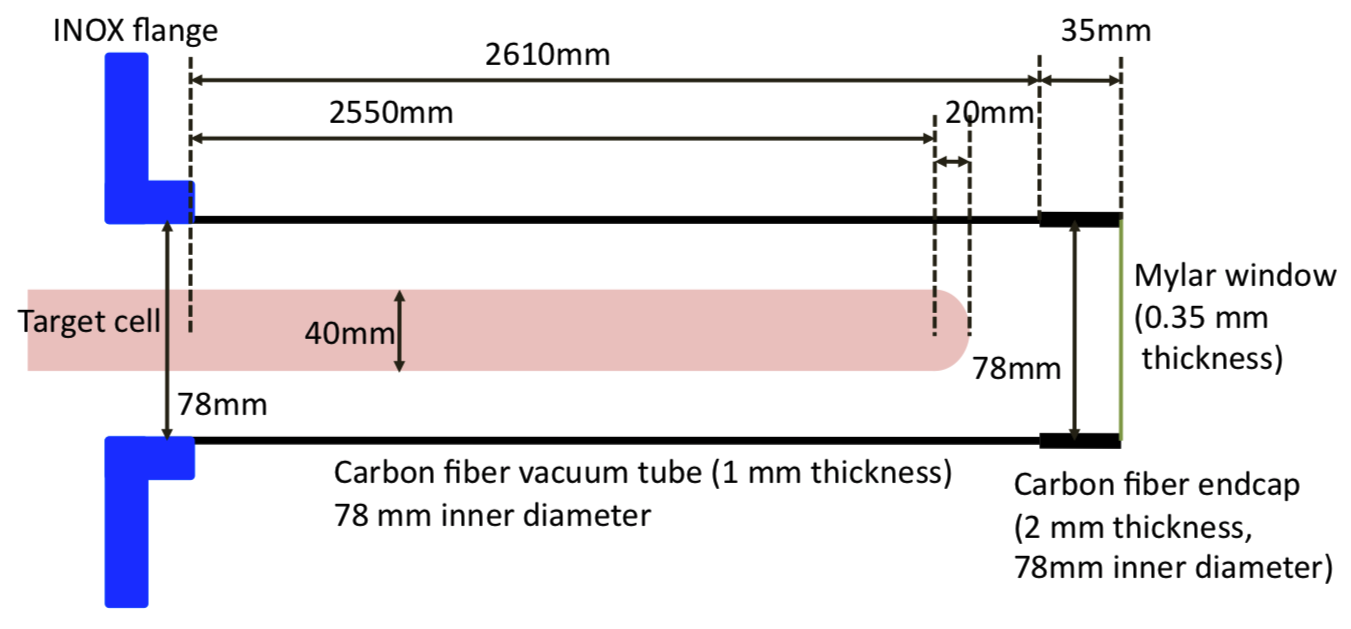
\includegraphics[scale=0.3]{./gfx/Target.png}
	\caption{Comparison of reconstructed Cherenkov angle as a function of the momentum with the calculated Cherenkov angle for each particle type using the refractive index of the RICH gas.}
	\label{pic:RefIndex}
\end{figure}

\section{Method}

The particle identification efficiency of the RICH is studied as a function of the hadron phase space, which is given by the hadron momentum and the polar angle at the entrance of the RICH. This was already studied before, for example in References \cite{} and \cite{}. The binning used for this study is similar to a previous analysis described in Reference \cite{}. A fine binning is used for the momentum dependence since the Cherenkov effect depends on this variable. For the dependence on the polar angle, a coarse binning is used, since only a weak dependence is observed. The binning is given by:

\begin{itemize}
  \item Momentum $p_h$ (GeV/c) : \{3,5,7,10,12,13,15,17,19,22,25,27,30,35,40,50\}
  \item Angle $\theta_h$ (rad) : \{0,0.01,0.04,0.12,0.3\}
\end{itemize}

For each bin, the elements of the efficiency matrix $M_R$ are determined separately for positive and negative particles. The elements of this matrix contain the probability for a particle $t$ to be identified as a particle of type $i$, for example a pion that is correctly identified as pion or wrongly as a kaon. The full matrix is given by:

\begin{equation}
  M_R
  =
  \begin{bmatrix}
  \epsilon(\pi \rightarrow \pi) & \epsilon(K \rightarrow \pi) & \epsilon(p \rightarrow \pi)\\
  \epsilon(\pi \rightarrow K) & \epsilon(K \rightarrow K) & \epsilon(p \rightarrow K) \\
  \epsilon(\pi \rightarrow p) & \epsilon(K \rightarrow p) & \epsilon(p \rightarrow p)
  \end{bmatrix}
\end{equation}

The different elements are determined by $\varepsilon(t \rightarrow i)$ = $N(t \rightarrow i)/N(t)$ where $N(t)$ is the total number of particles $t$ and $N(t \rightarrow i)$ is the number of particles $t$, which are identified as particle $i$. These numbers are evaluated using samples, where the particle type is known, as in the case of the selected decays. In the case of positive pions, the events from the $K^0$ sample are used where the negative hadron is identified as a pion using the likelihood cuts shown in Table. \ref{tab:LHcut}.  Therefore, the second particle has to be a pion too, if the decaying particle was a $K^0$. Using the RICH, the particle type is determined for the second particle, which  results in the number $N(\pi^+ \rightarrow i)$. An equivalent procedure is used for positive kaons and protons using the $\Phi$ and $\Lambda$ samples. In order to obtain these numbers for the negative particles, the same samples are used but this time performing the identification of the positive particle in the first place. The numbers $N(t \rightarrow i)$ are extracted using a fit, which is described here for the $K^0$ sample, where the negative pion is already identified. The events are put into five different groups, depending on the particle type determined by the RICH :

\begin{itemize}
  \item All events (RICH not used for second particle)
  \item Events where $\pi^+$ is identified as $\pi^+$
  \item Events where $\pi^+$ is identified as $K^+$
  \item Events where $\pi^+$ is identified as $p$
  \item Events where $\pi^+$ is not identified
\end{itemize}

For each of these groups, the invariant $K^0$ mass spectra are shown in Fig. \ref{pic:K0MassSpectra}, for example, and the number of events in the peak and the background are determined by a simultaneous fit of all five spectra. These spectra are described using two Gaussian distributions with the same mean for the signal, $f_{sig}$, and a polynomial to describe the background, $f_{bg}$. Their expressions are given in Table. \ref{tab:FunctionForm}. The two Gaussian distributions account for the different resolutions of the two spectrometer stages. The fitted function for each of the groups is given by

\begin{equation}
  f(x) = N_{sig} \dot f_{sig} + N_{bg} \dot f_{bg}
\end{equation}

where $N_{sig}$ is the amount of $K^0$ and $N_{bgd}$ the amount of background events. Here, the same width, $\sigma_1$ and $\sigma_2$, of the two Gaussian distributions was used for all five spectra.

\begin{table}[!h]
  \caption{Functional form for the descriptin of the mass spectra for $K^0$, $\Phi$ and $\Lambda$ candidates. The symbol $G$ represents a Gaussian distribution and the symbol $BW$ a relative Breit-Wigner distribution.}
  \label{tab:FunctionForm}
  \centering
  \begin{tabular}{lcc}
    \hline
    SAMPLE & SIGNAL & BACKGROUND \\
    \hline
    $K^0$ & $\delta G(\mu,\sigma_1) + (1-\delta)G(\mu,\sigma_2)$ & $1+ax+b(2x^2-1)+c(4x^3-3x)$ \\
    $\Phi$ & $BW(\mu,\sigma_1) \otimes G(\mu,\sigma_2)$ & $(x-t)^n \cdot exp(-a(x-t))$ with $t=2 \cdot m_K$ \\
    $\Lambda$ & $\delta G(\mu,\sigma_1) + (1-\delta)G(\mu,\sigma_2)$ & $(x-t)^n \cdot exp(-a(x-t))$ with $t= m_p + m_{\pi}$ \\
    \hline
  \end{tabular}
\end{table}

\begin{figure}[!h]
  \centering
	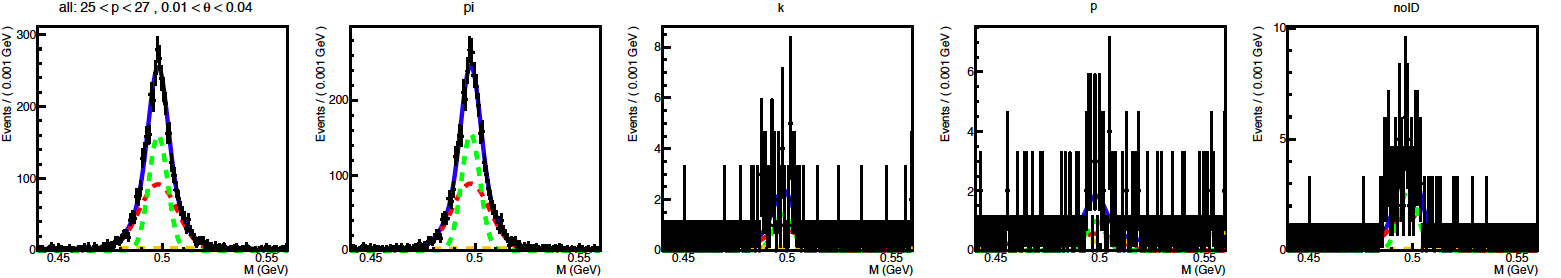
\includegraphics[scale=0.3]{./gfx/K0MassSpectra.png}
	\caption{Mass spectra for $K^0$ candidates with an identified $\pi^-$ for various hypotheses for the second hadron (from left to right : all, $\pi$, $K$, $p$, no ID). The momentum of the positive hadron is in the range of [25,27] GeV/$c^2$ and in the angle in the range [0.01,0.04].}
	\label{pic:K0MassSpectra}
\end{figure}

Also the ratio $\delta$ of the amount of events in both Gaussian distributions is the same. The shape of the background is the same for all spectra except the one where the pion is identified as a proton. In this case, a possible background contribution due to decays from $\Lambda$ baryons decaying in a pion and an proton can be enriched. This results in  a slightly different background shape. The integral of the background remains a independent parameter in all five cases. In order to ensure that the sum of all efficiencies  ($\varepsilon(\pi^+ \rightarrow \pi^+)  + \varepsilon(\pi^+ \rightarrow K^+ ) + \varepsilon(\pi^+ \rightarrow p ) + \varepsilon(\pi^+ \rightarrow noID)$) is 100\%, an additional constraint is introduced to the fit.

\begin{equation}
  N^{all}(K^0) = N^{\pi}(K^0) + N^{K}(K^0) + N^{p}(K^0) + N^{noID}(K^0)
\end{equation}

where $N_i(K^0)$ (i = $\pi$, $K$, $p$, $noID$) is the number of $K^0$ obtained from the histogram where the pion is identified as $i$. This results in 16 free parameters of the fit. The same method is used in the case of kaons and protons. The main difference between those fits and the one for the $K^0$ sample is the description of the signal and the background. The functions describing both are also given in Table. \ref{tab:FunctionForm}. Again the parameters describing the shape are the same in all five spectra and the fit parameters  describing the integrals of the functions are used as free parameters, except for the parameter of the mass spectrum including all events. This results in 15 free parameters for the fit of the $\Phi$ sample and in 15 free parameters for the fit of the $\Lambda$ sample. Examples of the fits performed for the $\Phi$ and $\Lambda$ samples are shown in Figs. \ref{pic:PhiMassSpectra} and \ref{pic:LambdaMassSpectra}. The fits show the results for one momentum bin (25 GeV/c2 $< p <$ 27 GeV/c2) and angular bin (0.01 $< \theta <$ 0.04), which was also shown for the $K^0$ sample.

\begin{figure}[!h]
  \centering
	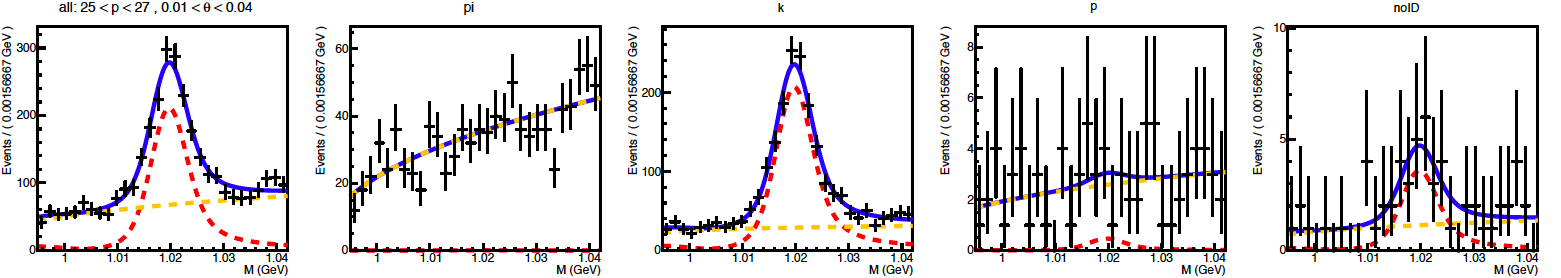
\includegraphics[scale=0.3]{./gfx/PhiMassSpectra.png}
	\caption{Mass spectra for $\Phi$ candidates with an identified $K^-$ for various hypotheses for the second hadron (from left to right : all, $\pi$, $K$, $p$, no ID). The momentum of the positive hadron is in the range of [25,27] GeV/$c^2$ and in the angle in the range [0.01,0.04].}
	\label{pic:PhiMassSpectra}
\end{figure}

\begin{figure}[!h]
  \centering
	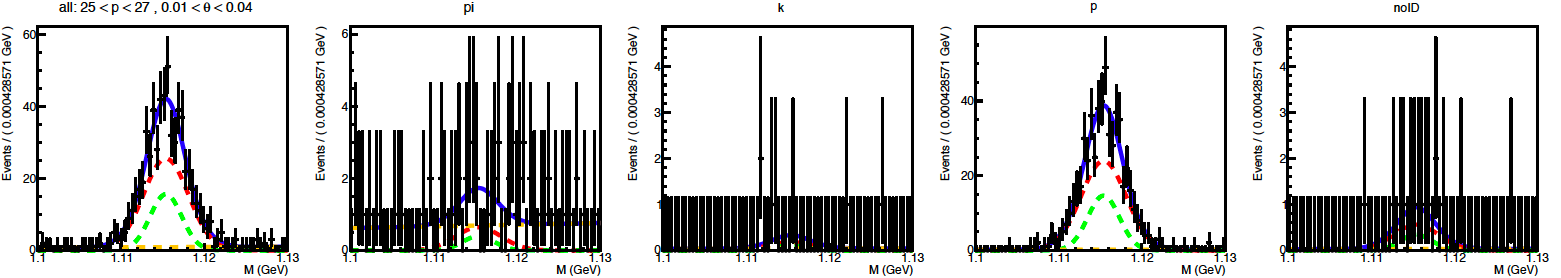
\includegraphics[scale=0.3]{./gfx/LambdaMassSpectra.png}
	\caption{Mass spectra for $\Lambda$ candidates with an identified $\pi^-$ for various hypotheses for the second hadron (from left to right : all, $\pi$, $K$, $p$, no ID). The momentum of the positive hadron is in the range of [25,27] GeV/$c^2$ and in the angle in the range [0.01,0.04].}
	\label{pic:LambdaMassSpectra}
\end{figure}

\section{Calculation of the efficiencies and uncertainties}

The elements of the efficiency matrix $M_R$ are determined from fitted numbers of signal events,

\begin{equation}
  \epsilon(t\rightarrow i) = \frac{N(t\rightarrow i)}{N(t)}
\end{equation}

Here, $N(t)$ is given by the sum of all $N(t \rightarrow i)$. As the nominator and denominator are correlated, the uncertainty can be determined via error propagation taking into account the covariance matrix of the fit,

\begin{equation}
  \Delta \epsilon = \sqrt{\sum_{j=1}^m \left( \frac{\delta \epsilon}{\delta N(i\rightarrow j)} \right)^2 \cdot u_j + 2 \sum_{j=1}^{m-1} \sum_{k=j+1}^{m} \left( \frac{\delta \epsilon}{\delta N(i\rightarrow j)} \frac{\delta \epsilon}{\delta N(i\rightarrow k)} \cdot u(j,k) \right)}
\end{equation}

where $u_j$ are the diagonal elements of the covariance matrix, $u(i,j)$ are the off diagonal elements and $\epsilon$ is one of the elements of the efficiency matrix. The summations are done over all possible particle types viz. pion, kaon, proton and non identified.

\section{Results}

The results for the RICH particle identification efficiency are shown in Figs. \ref{pic:Effpip} to \ref{pic:Effpb} for the various particle types and charges for the stricter likelihood cuts. In each figure, the momentum dependence for the different angular bins is shown. The efficiencies are weakly dependent on the angle while it is more strongly correlated with the momentum, especially in the region near the threshold.
The RICH performs a correct identification of pions in more than 95\% of the cases for momenta below 30 GeV/$c^2$ and the probability for a misidentification of a pion as a kaon is below $\sim$ 1\%. For kaons, near the threshold, a strong momentum dependence of the efficiencies is observed. At higher momenta the correct identification is given in $\sim$ 95\% of the cases. For protons, the momentum dependence around threshold level is even stronger. Below the threshold, protons are identified correctly in 50\% of the cases. Above the threshold numbers rise to $\sim$ 95\%. When using less strict likelihood cuts, the results are similar (Figs. \ref{pic:Lesspi+} to \ref{pic:Lesspb}). The correct identification of pions below 30 GeV/$c^2$ is done in 95\% of the cases. Due to less strict likelihood cuts the misidentification of pions as kaons is a bit larger but still below 3\% for momenta higher than 30 GeV/$c^2$. For a larger momenta a larger fraction of pions is identified as kaons, which got no identification for stricter cuts. For kaons and protons the results are similar : the probability of correct identification for kaons is a bit smaller but still above 95\%.

\begin{figure}[!p]
  \centering
	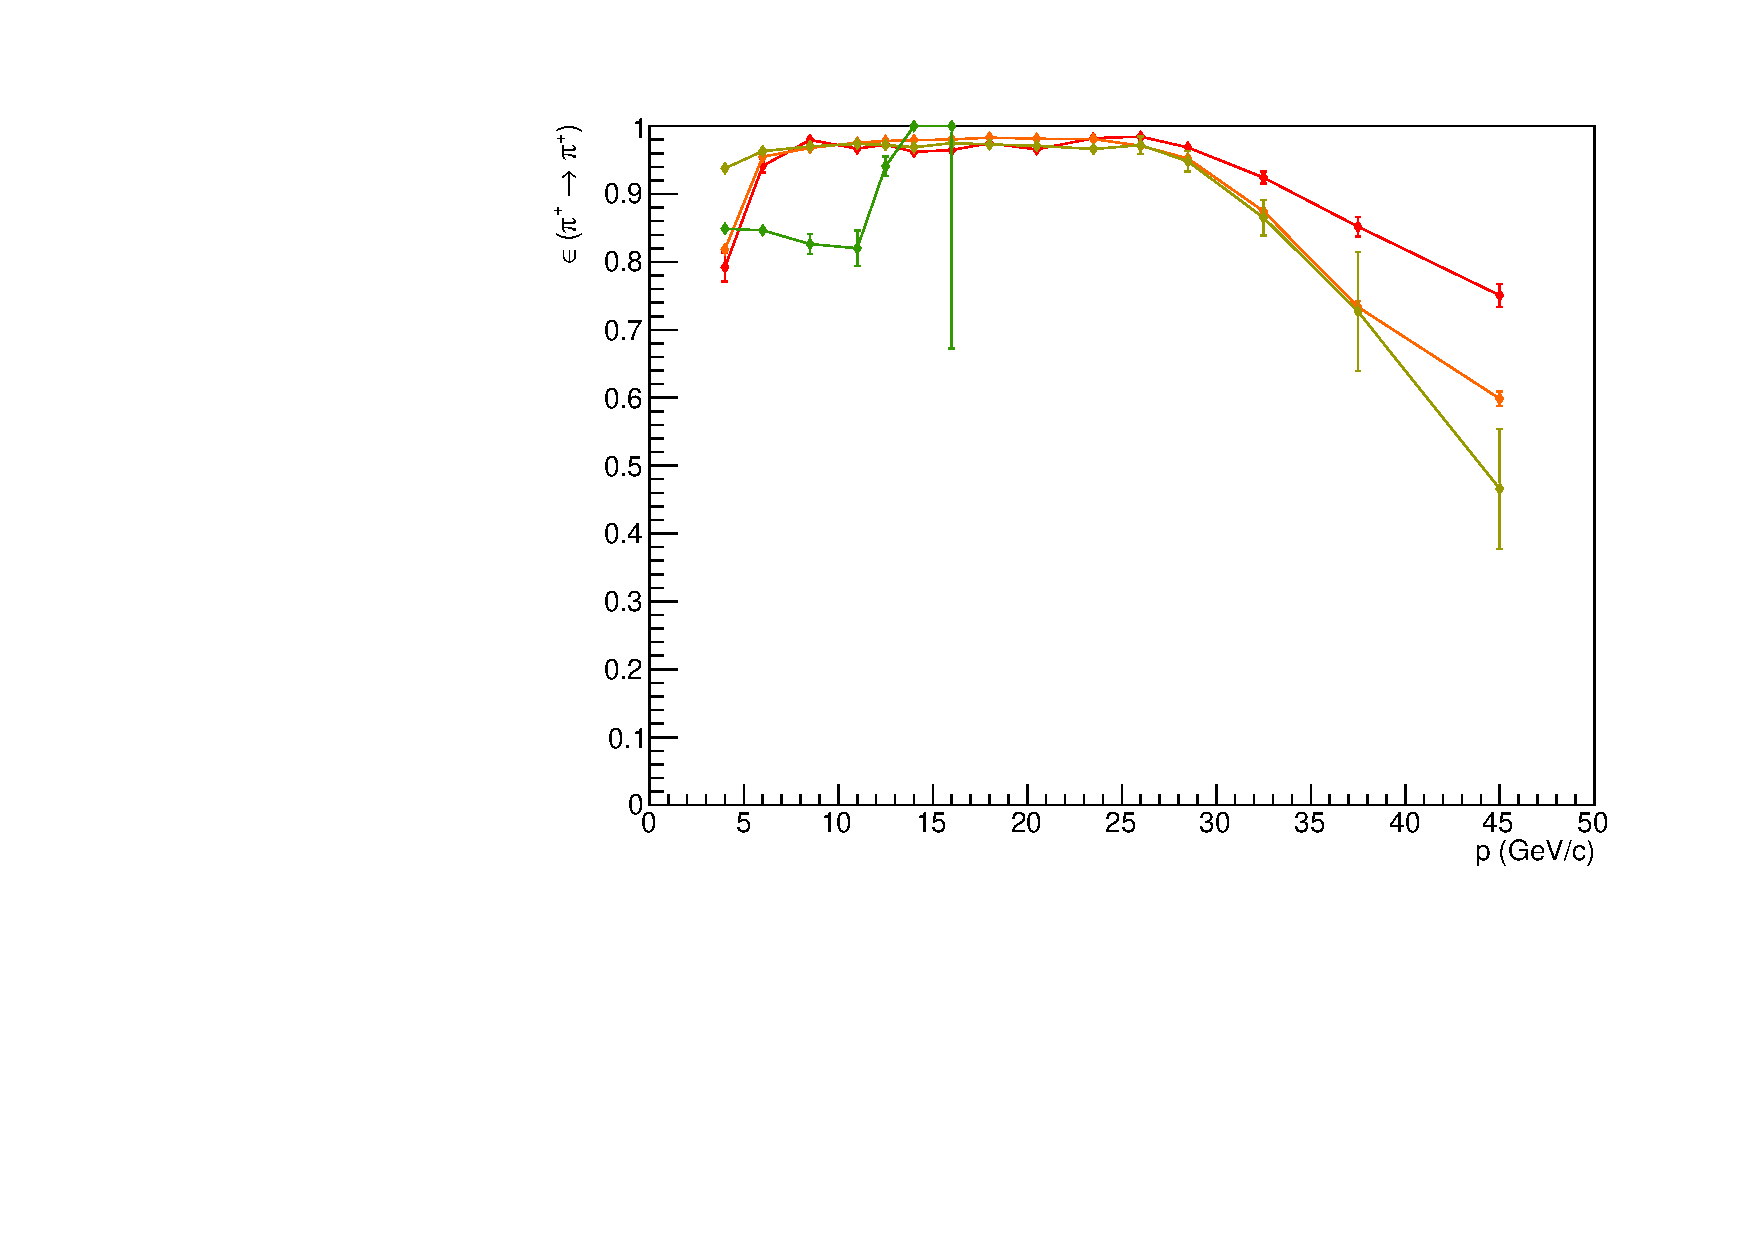
\includegraphics[scale=0.38]{./gfx/pip_pi.pdf}
  \includegraphics[scale=0.38]{./gfx/pip_K.pdf}
  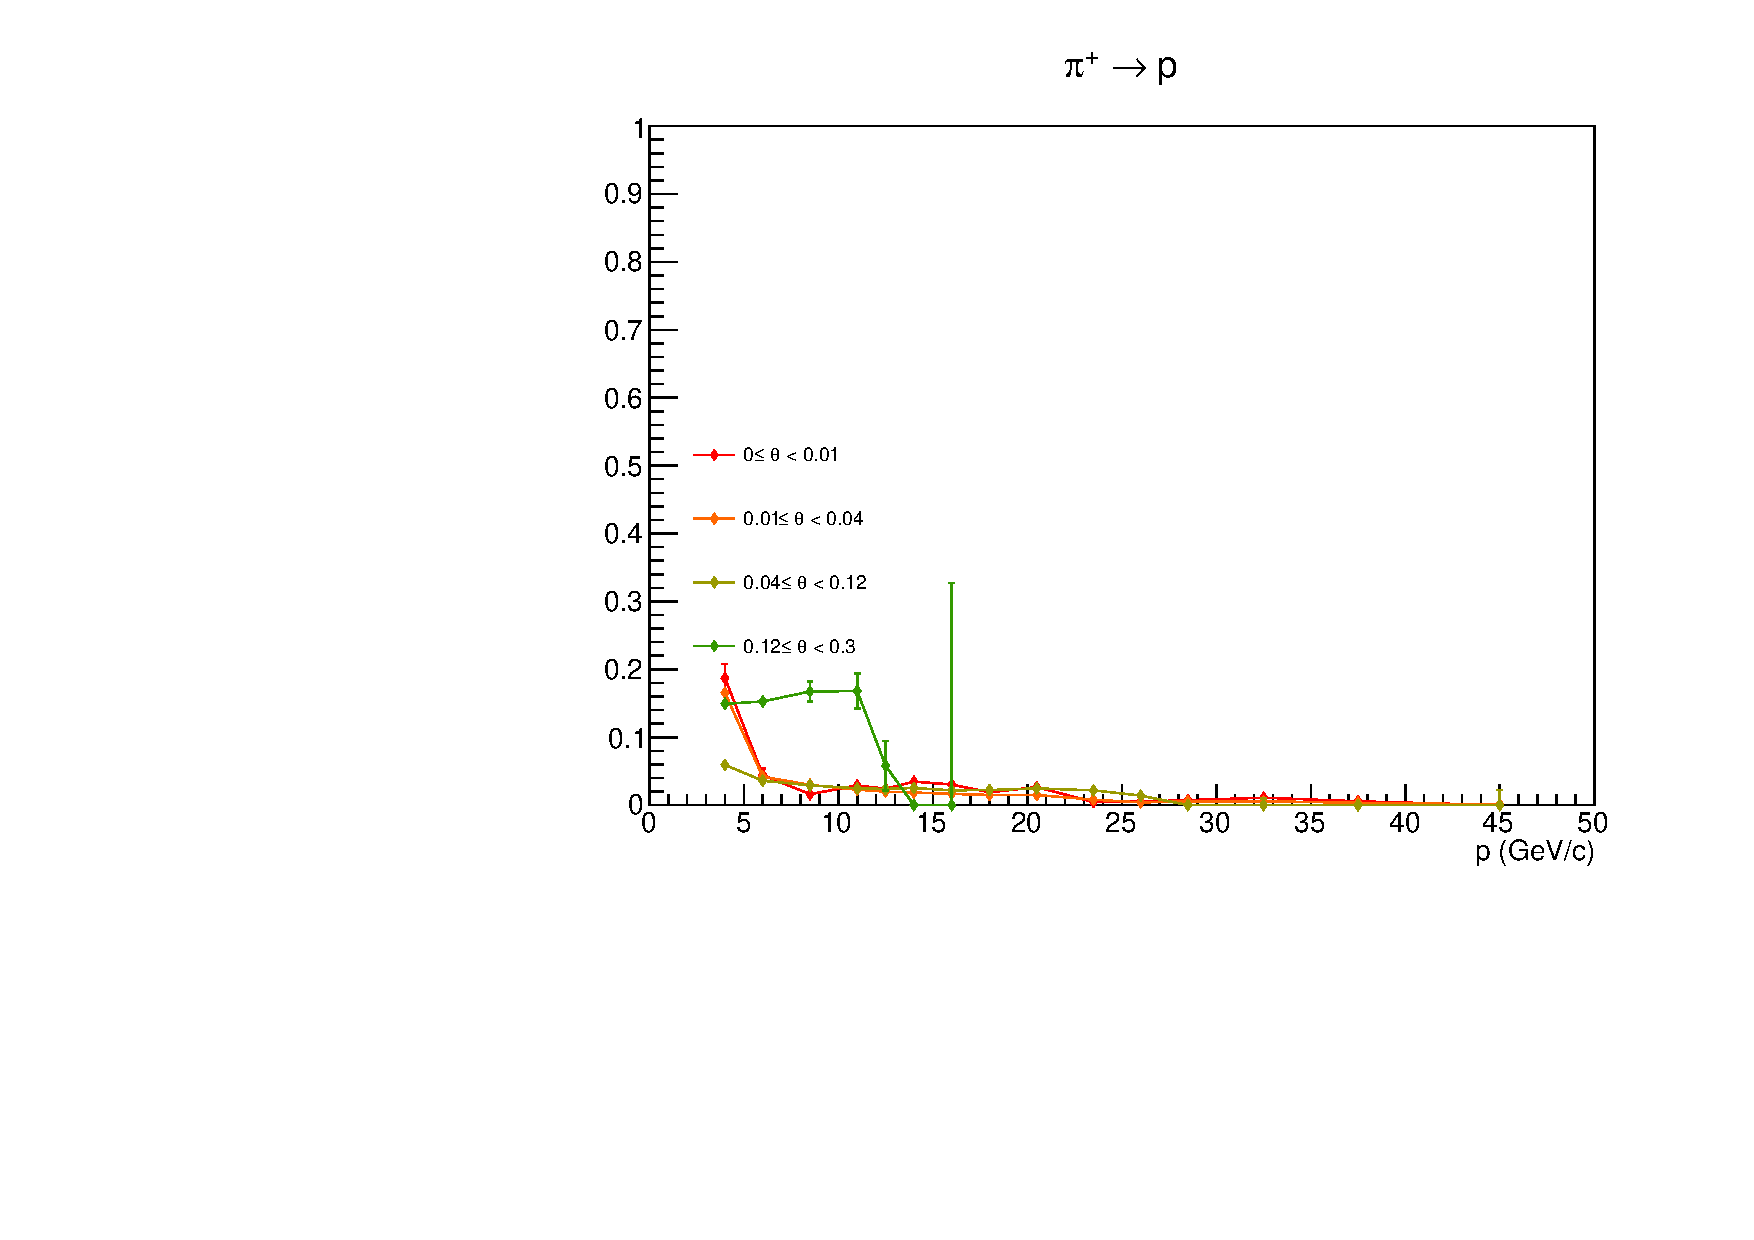
\includegraphics[scale=0.38]{./gfx/pip_p.pdf}
  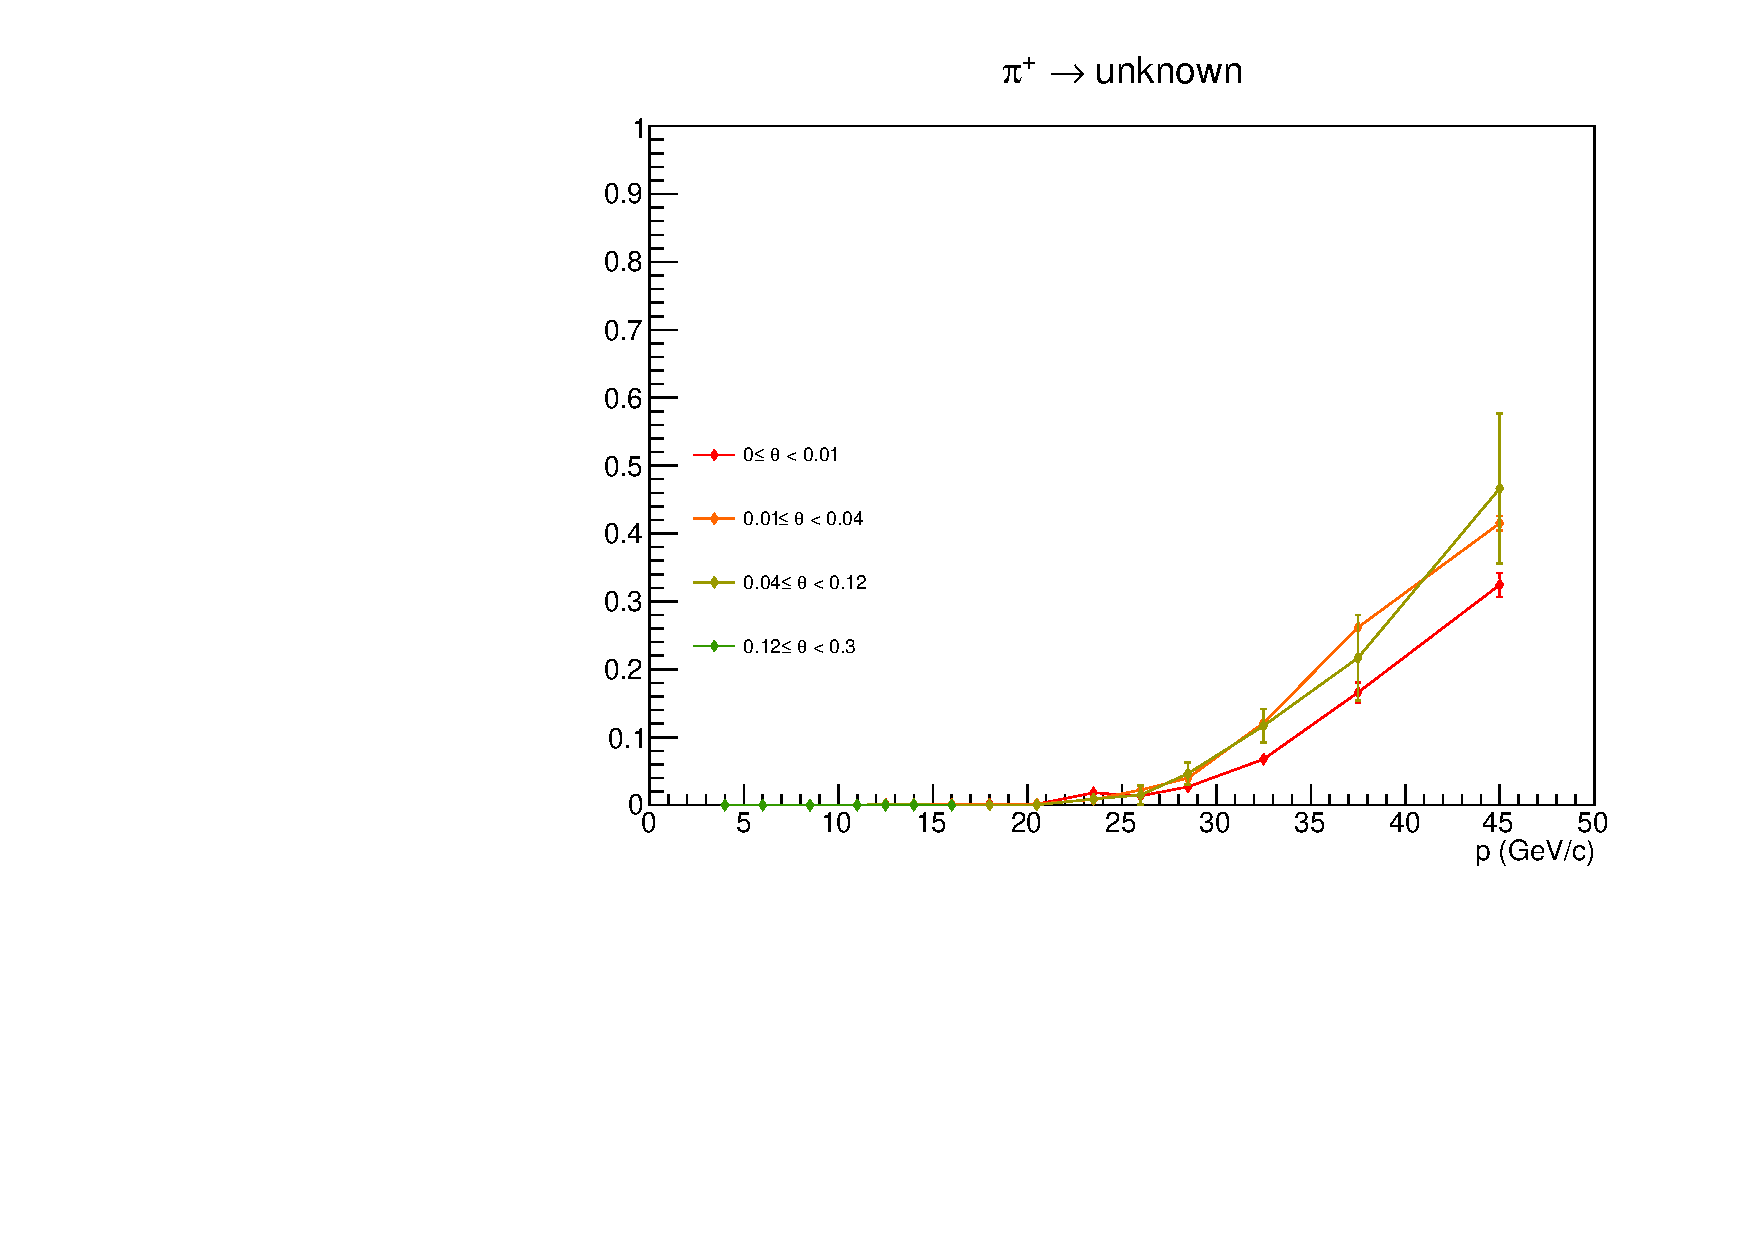
\includegraphics[scale=0.38]{./gfx/pip_u.pdf}
	\caption{Identification probabilities $\epsilon(p \rightarrow j)$ for $\pi^+$.}
	\label{pic:Effpip}
\end{figure}

\begin{figure}[!p]
  \centering
	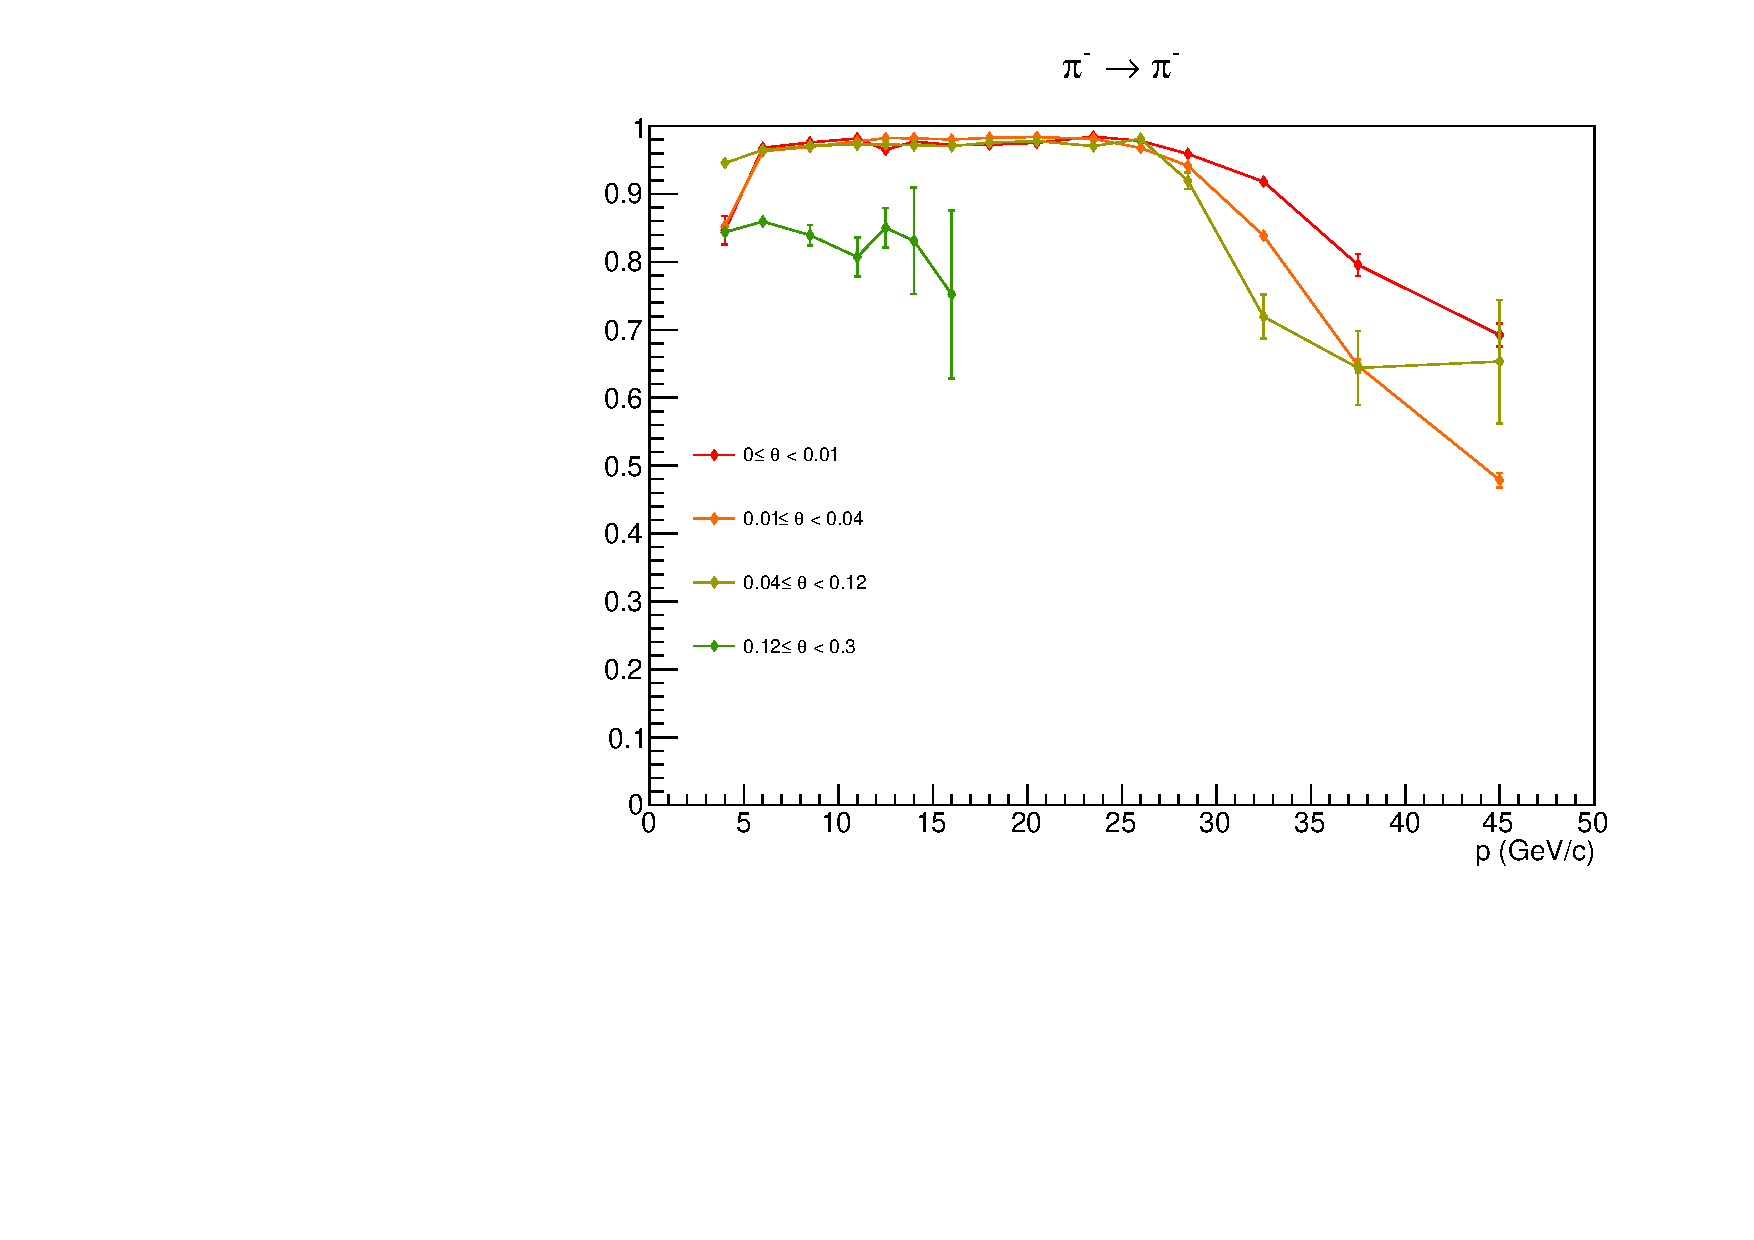
\includegraphics[scale=0.38]{./gfx/pim_pi.pdf}
  \includegraphics[scale=0.38]{./gfx/pim_K.pdf}
  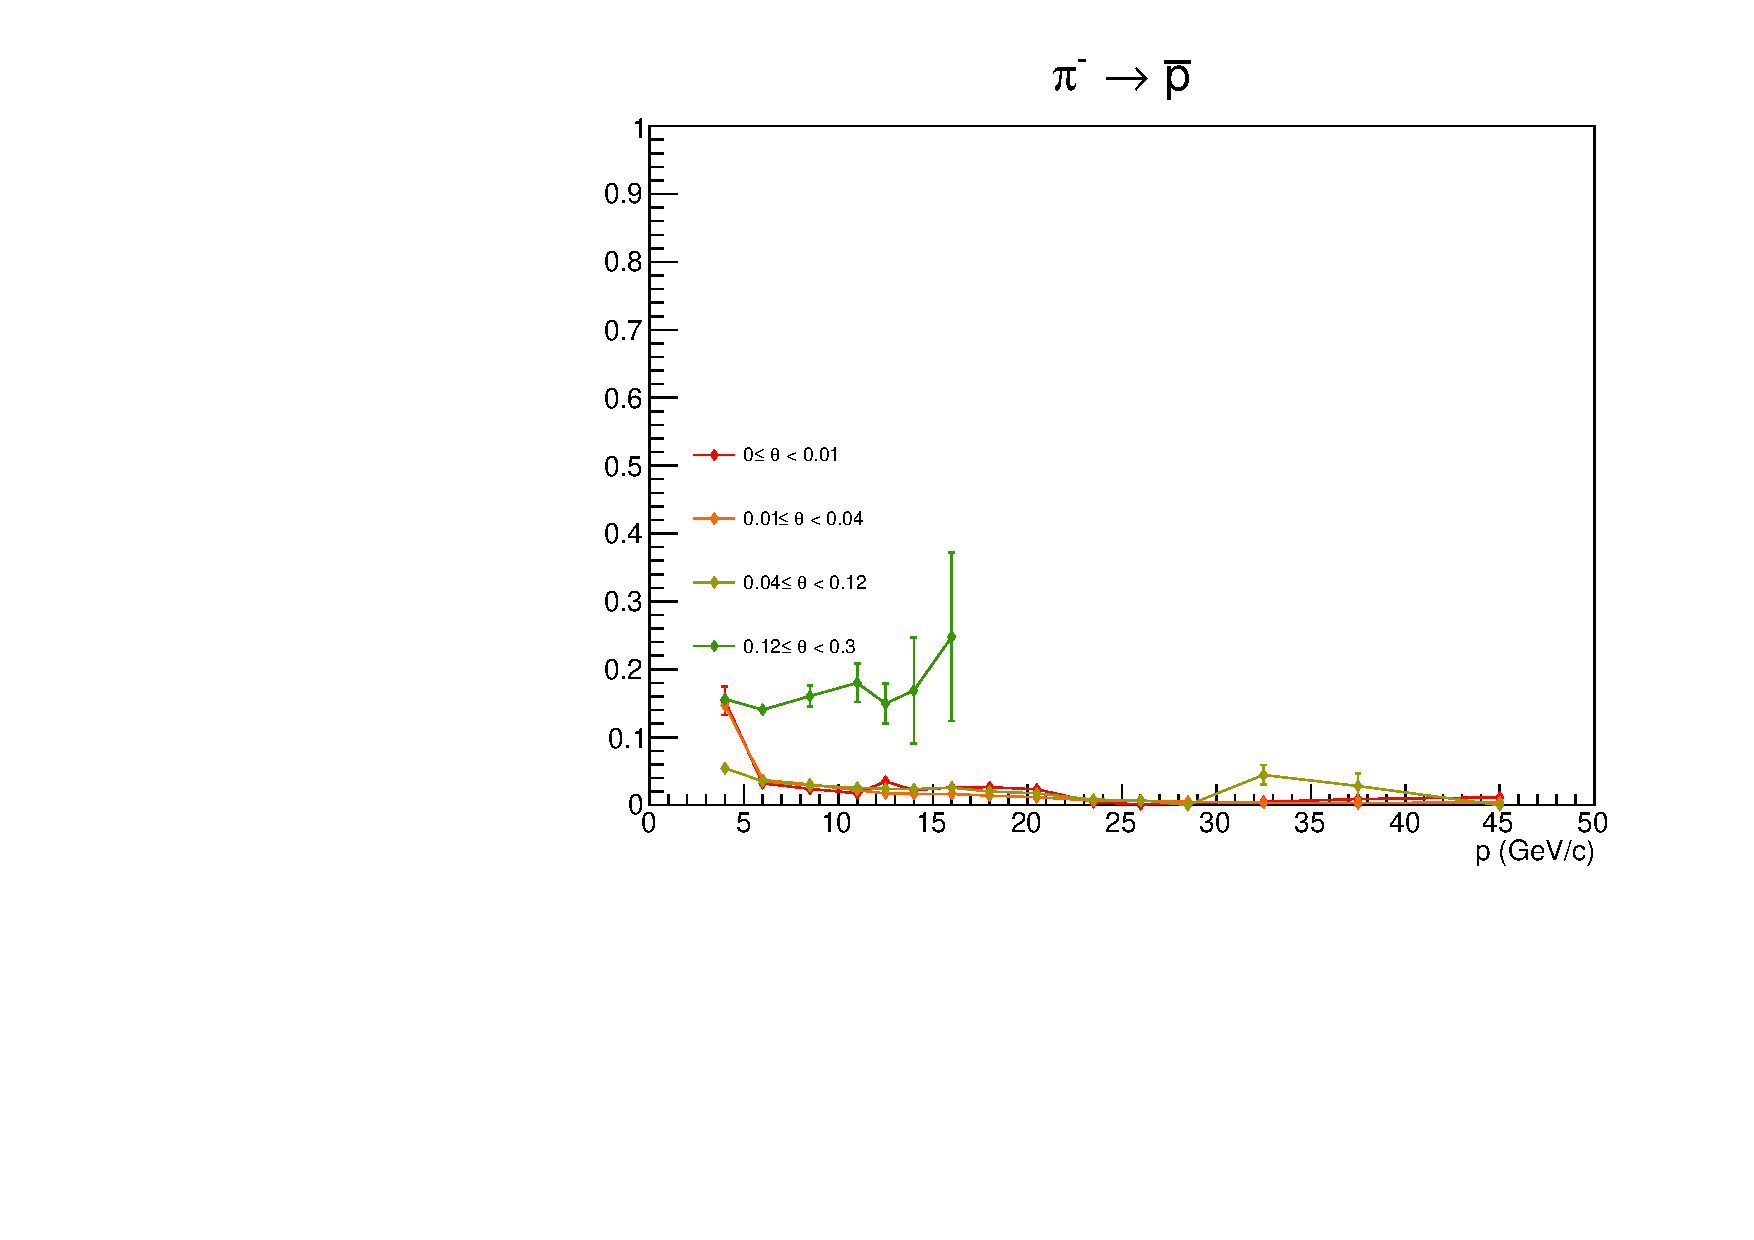
\includegraphics[scale=0.38]{./gfx/pim_p.pdf}
  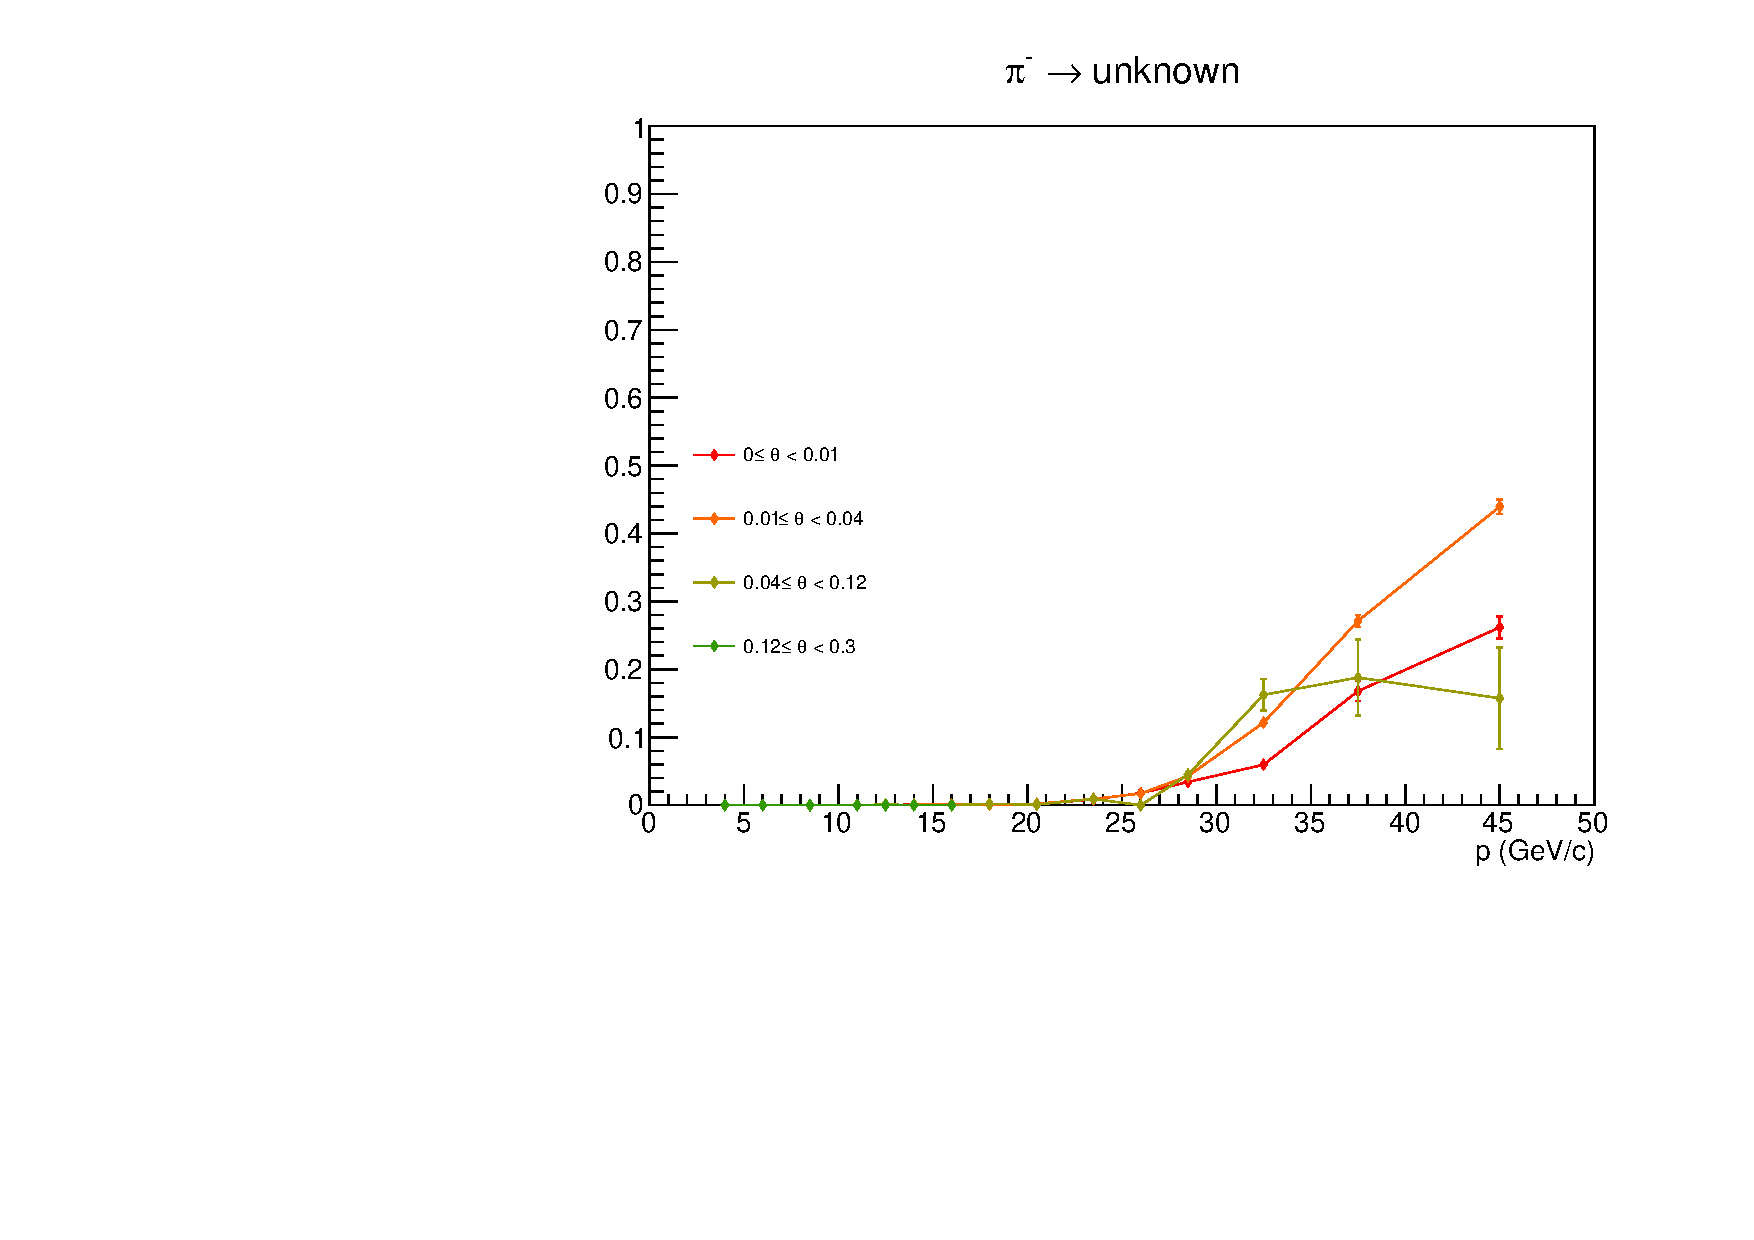
\includegraphics[scale=0.38]{./gfx/pim_u.pdf}
	\caption{Identification probabilities $\epsilon(p \rightarrow j)$ for $\pi^-$.}
	\label{pic:Effpim}
\end{figure}

\begin{figure}[!p]
  \centering
	\includegraphics[scale=0.38]{./gfx/Kp_pi.pdf}
  \includegraphics[scale=0.38]{./gfx/Kp_K.pdf}
  \includegraphics[scale=0.38]{./gfx/Kp_p.pdf}
  \includegraphics[scale=0.38]{./gfx/Kp_u.pdf}
	\caption{Identification probabilities $\epsilon(p \rightarrow j)$ for $K^+$.}
	\label{pic:Effpip}
\end{figure}

\begin{figure}[!p]
  \centering
	\includegraphics[scale=0.38]{./gfx/Km_pi.pdf}
  \includegraphics[scale=0.38]{./gfx/Km_K.pdf}
  \includegraphics[scale=0.38]{./gfx/Km_p.pdf}
  \includegraphics[scale=0.38]{./gfx/Km_u.pdf}
	\caption{Identification probabilities $\epsilon(p \rightarrow j)$ for $K^-$.}
	\label{pic:Effpim}
\end{figure}

\begin{figure}[!p]
  \centering
	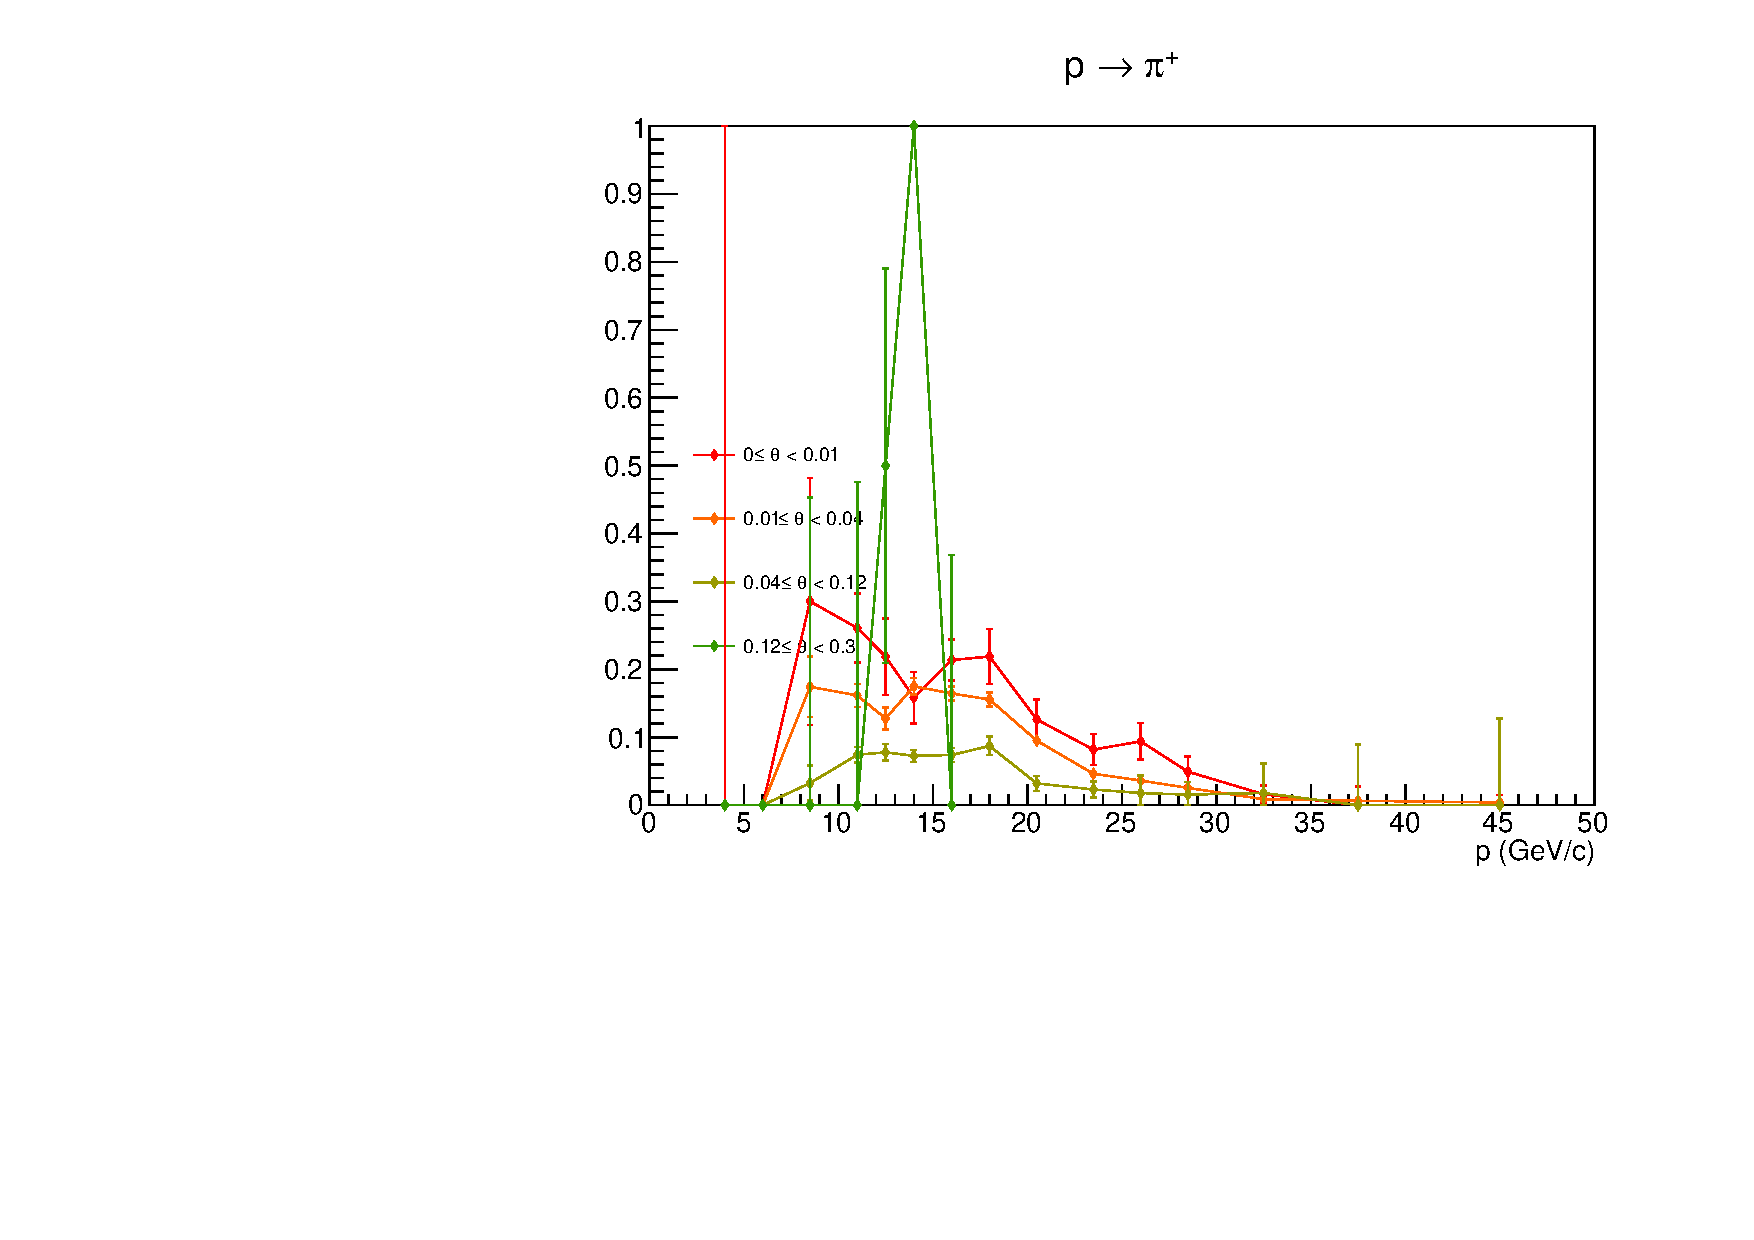
\includegraphics[scale=0.38]{./gfx/pp_pi.pdf}
  \includegraphics[scale=0.38]{./gfx/pp_K.pdf}
  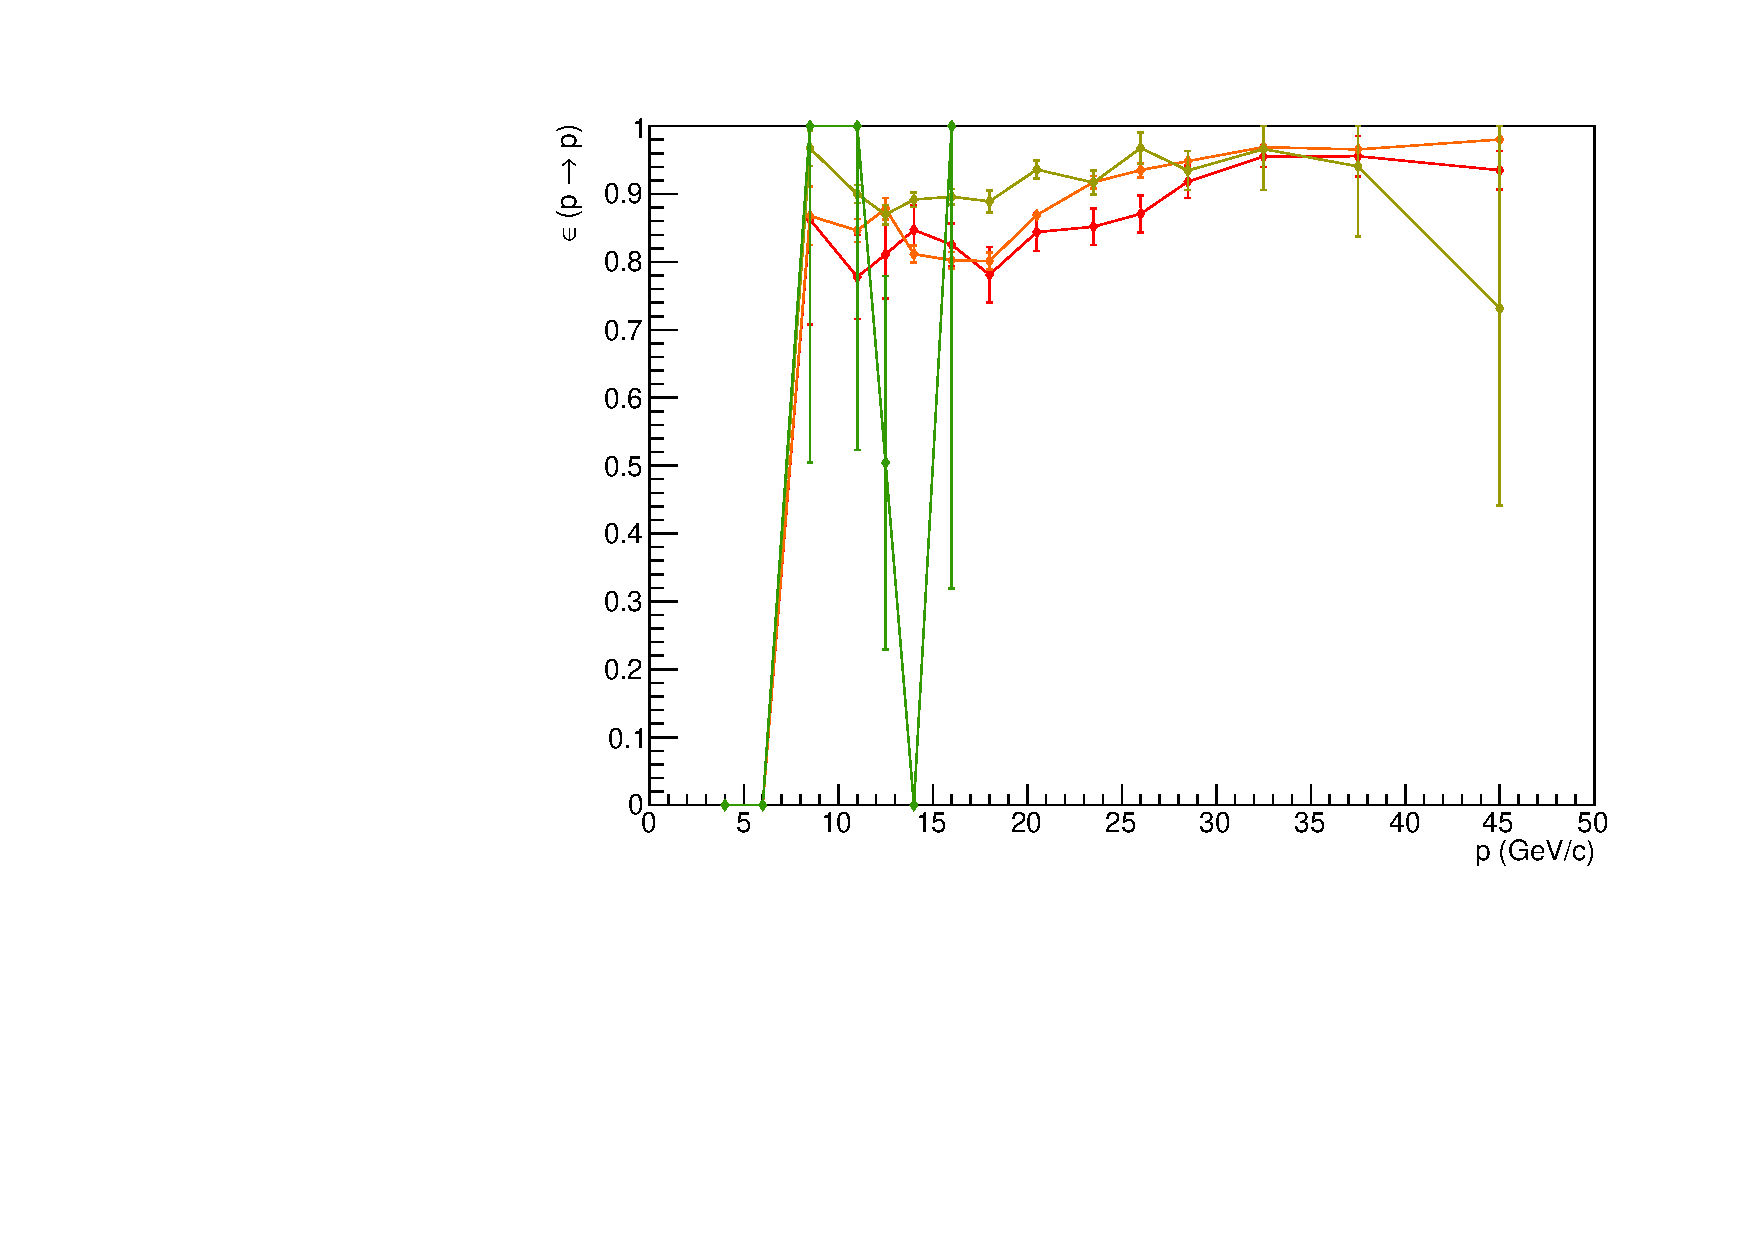
\includegraphics[scale=0.38]{./gfx/pp_p.pdf}
  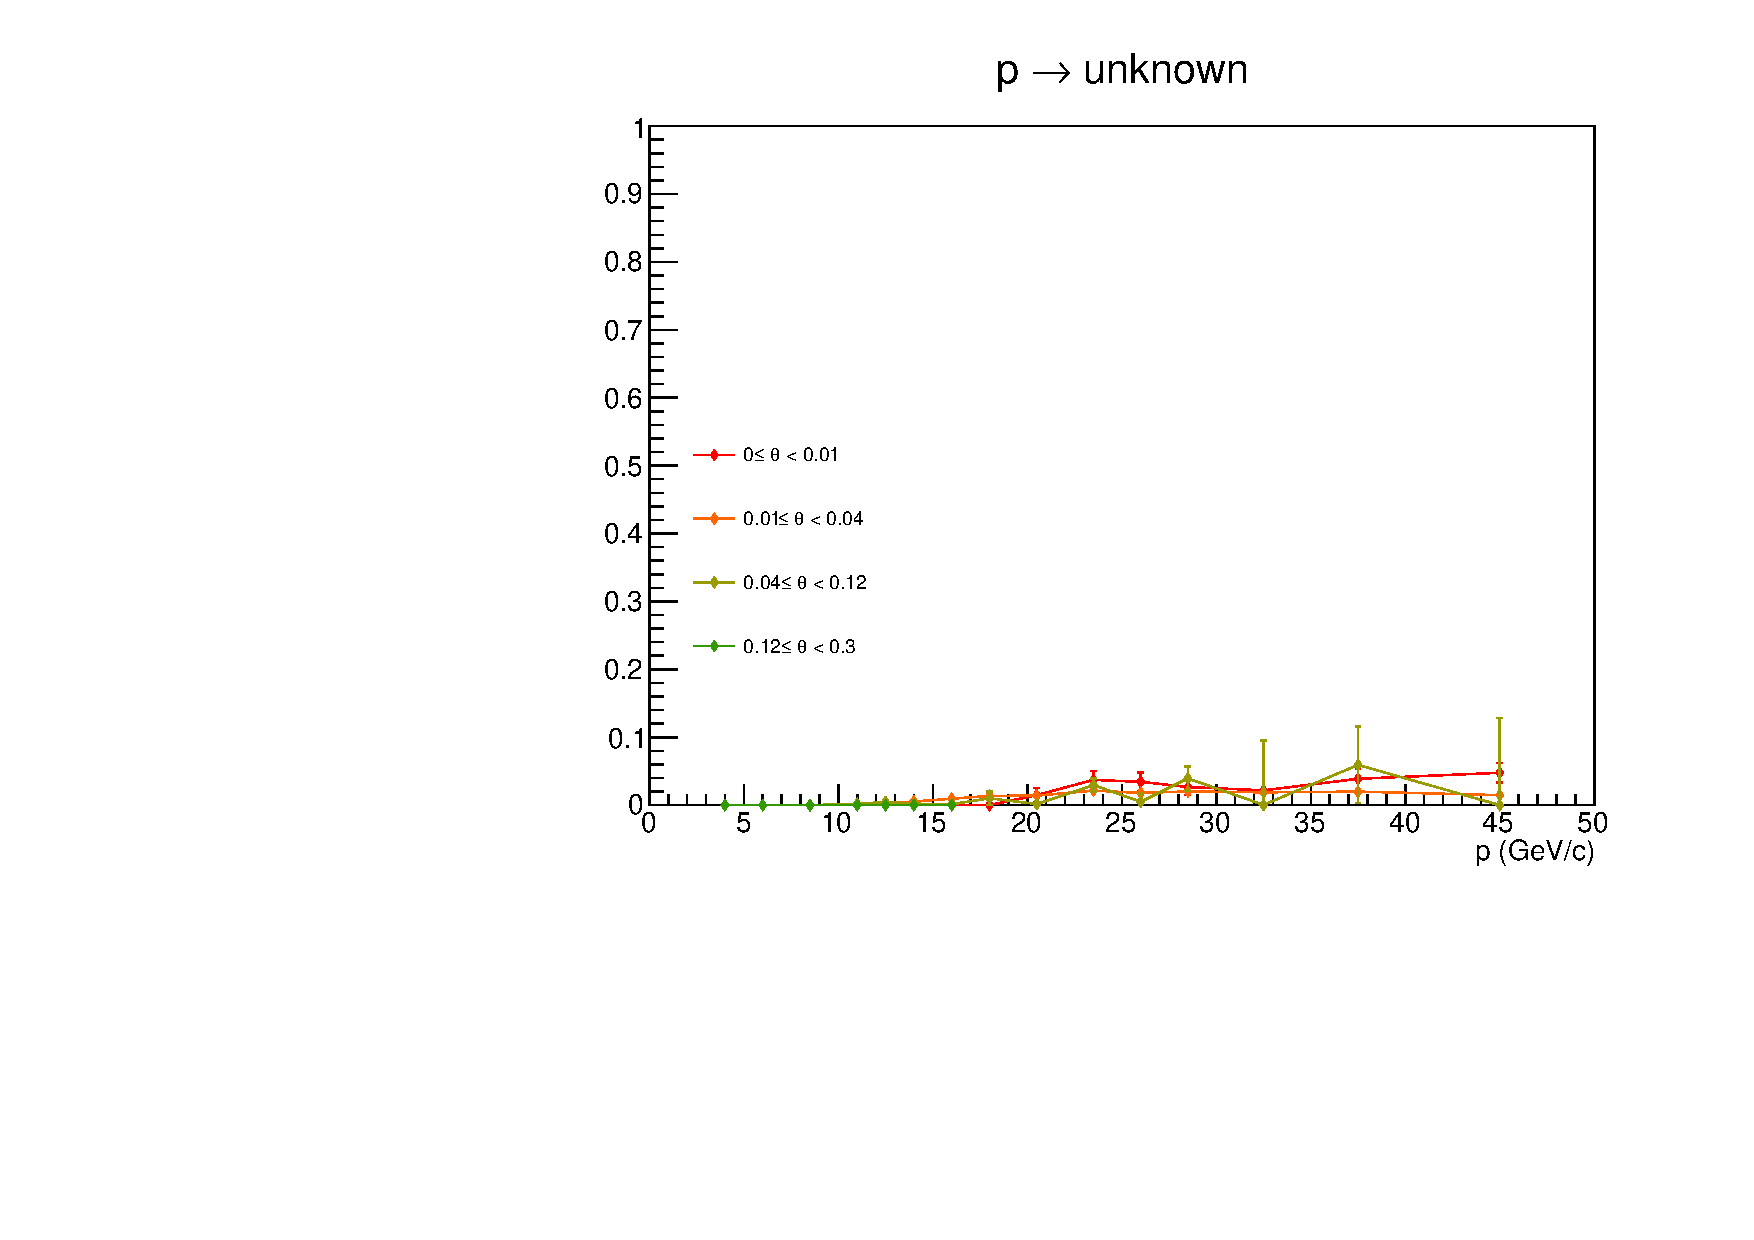
\includegraphics[scale=0.38]{./gfx/pp_u.pdf}
	\caption{Identification probabilities $\epsilon(p \rightarrow j)$ for $p$.}
	\label{pic:Effpip}
\end{figure}

\begin{figure}[!p]
  \centering
	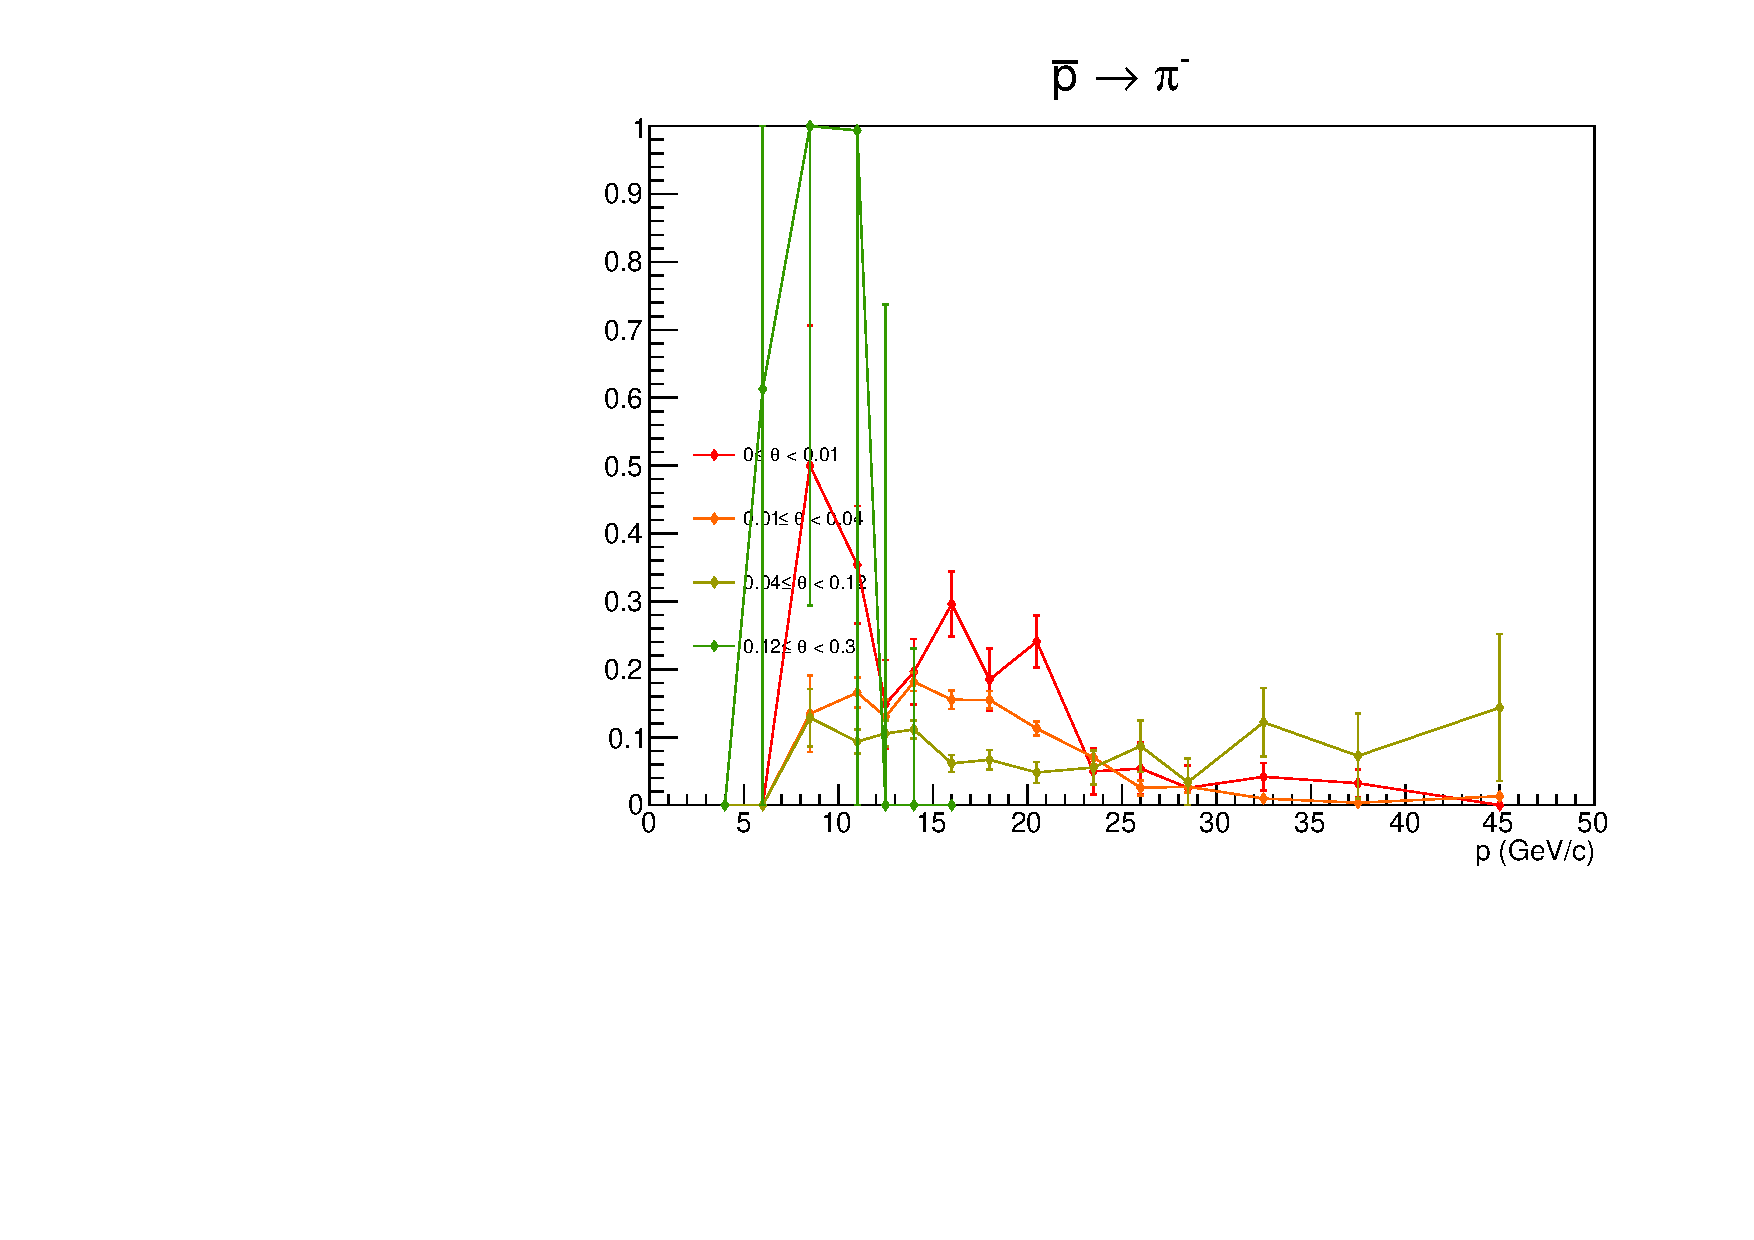
\includegraphics[scale=0.38]{./gfx/pm_pi.pdf}
  \includegraphics[scale=0.38]{./gfx/pm_K.pdf}
  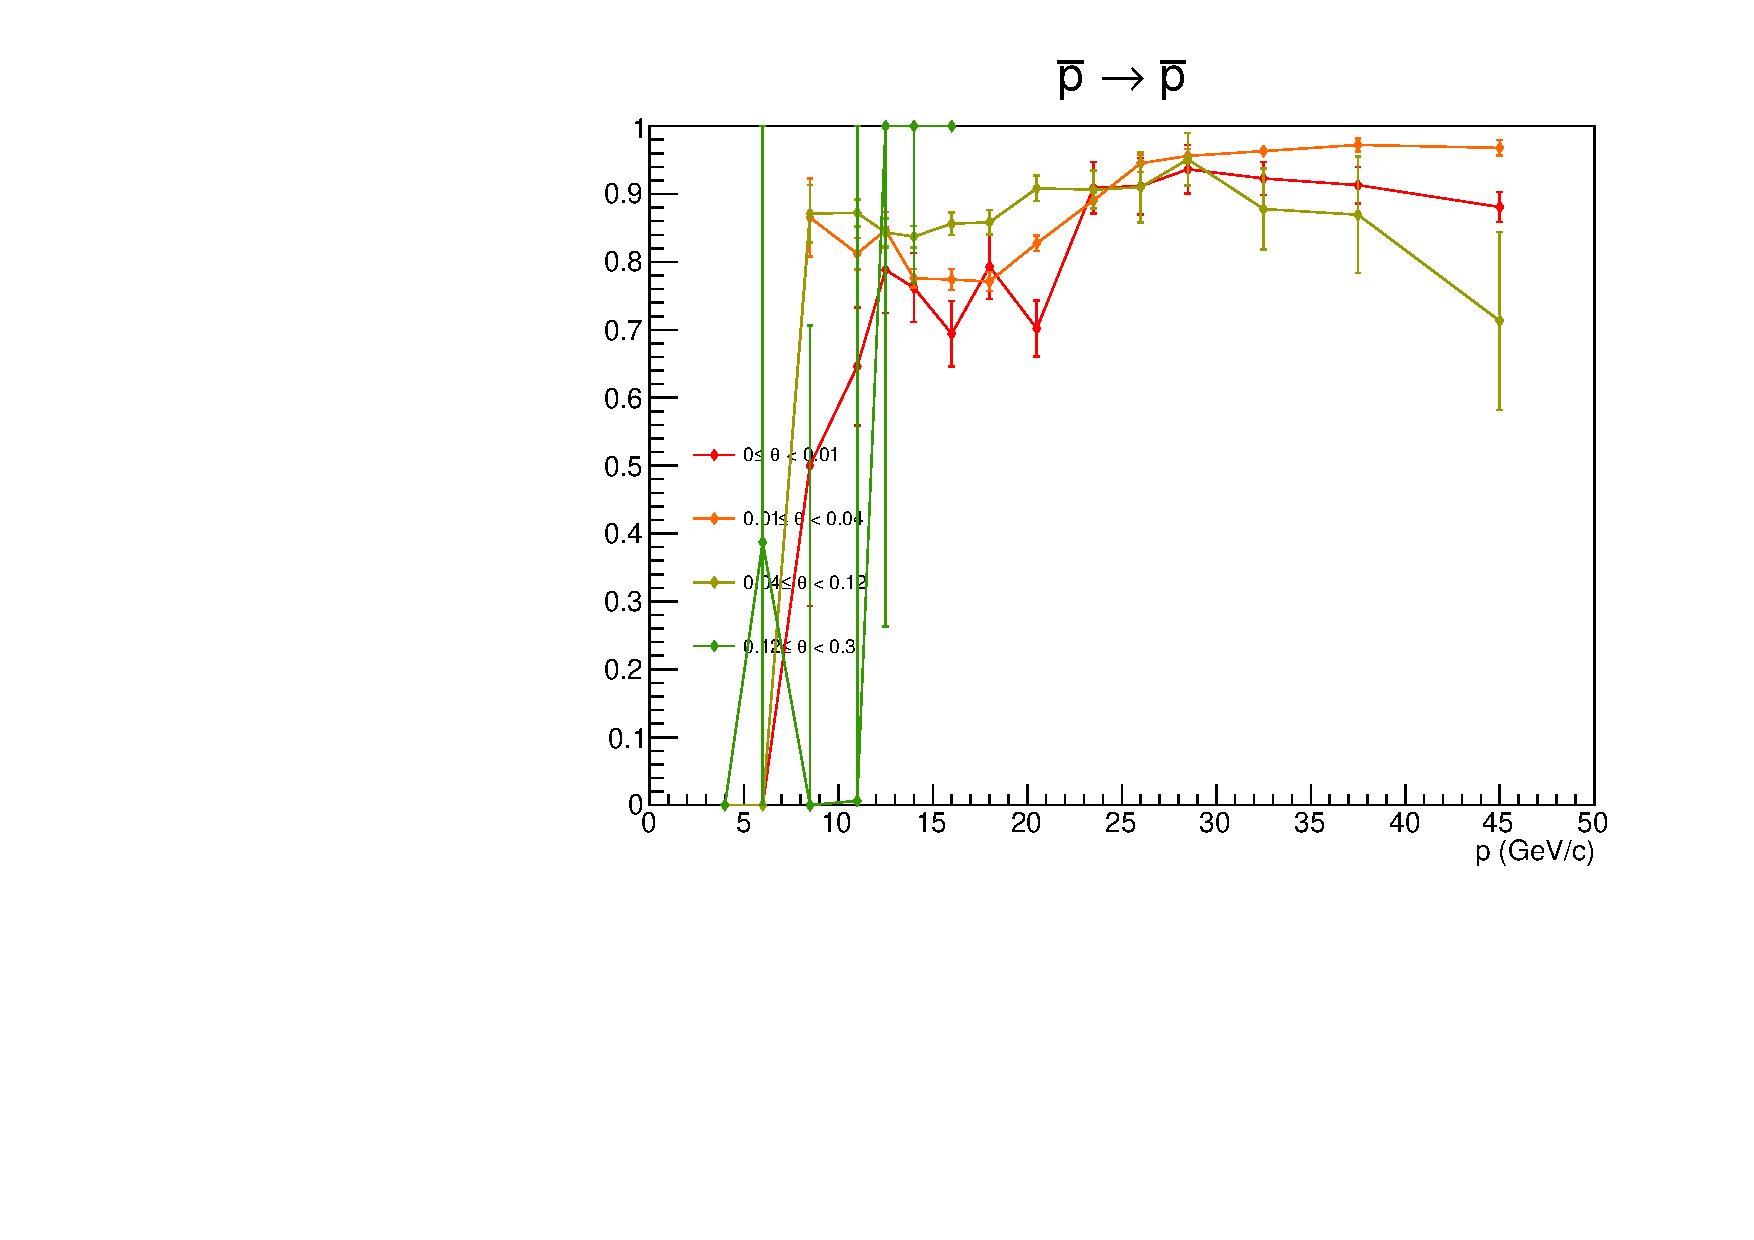
\includegraphics[scale=0.38]{./gfx/pm_p.pdf}
  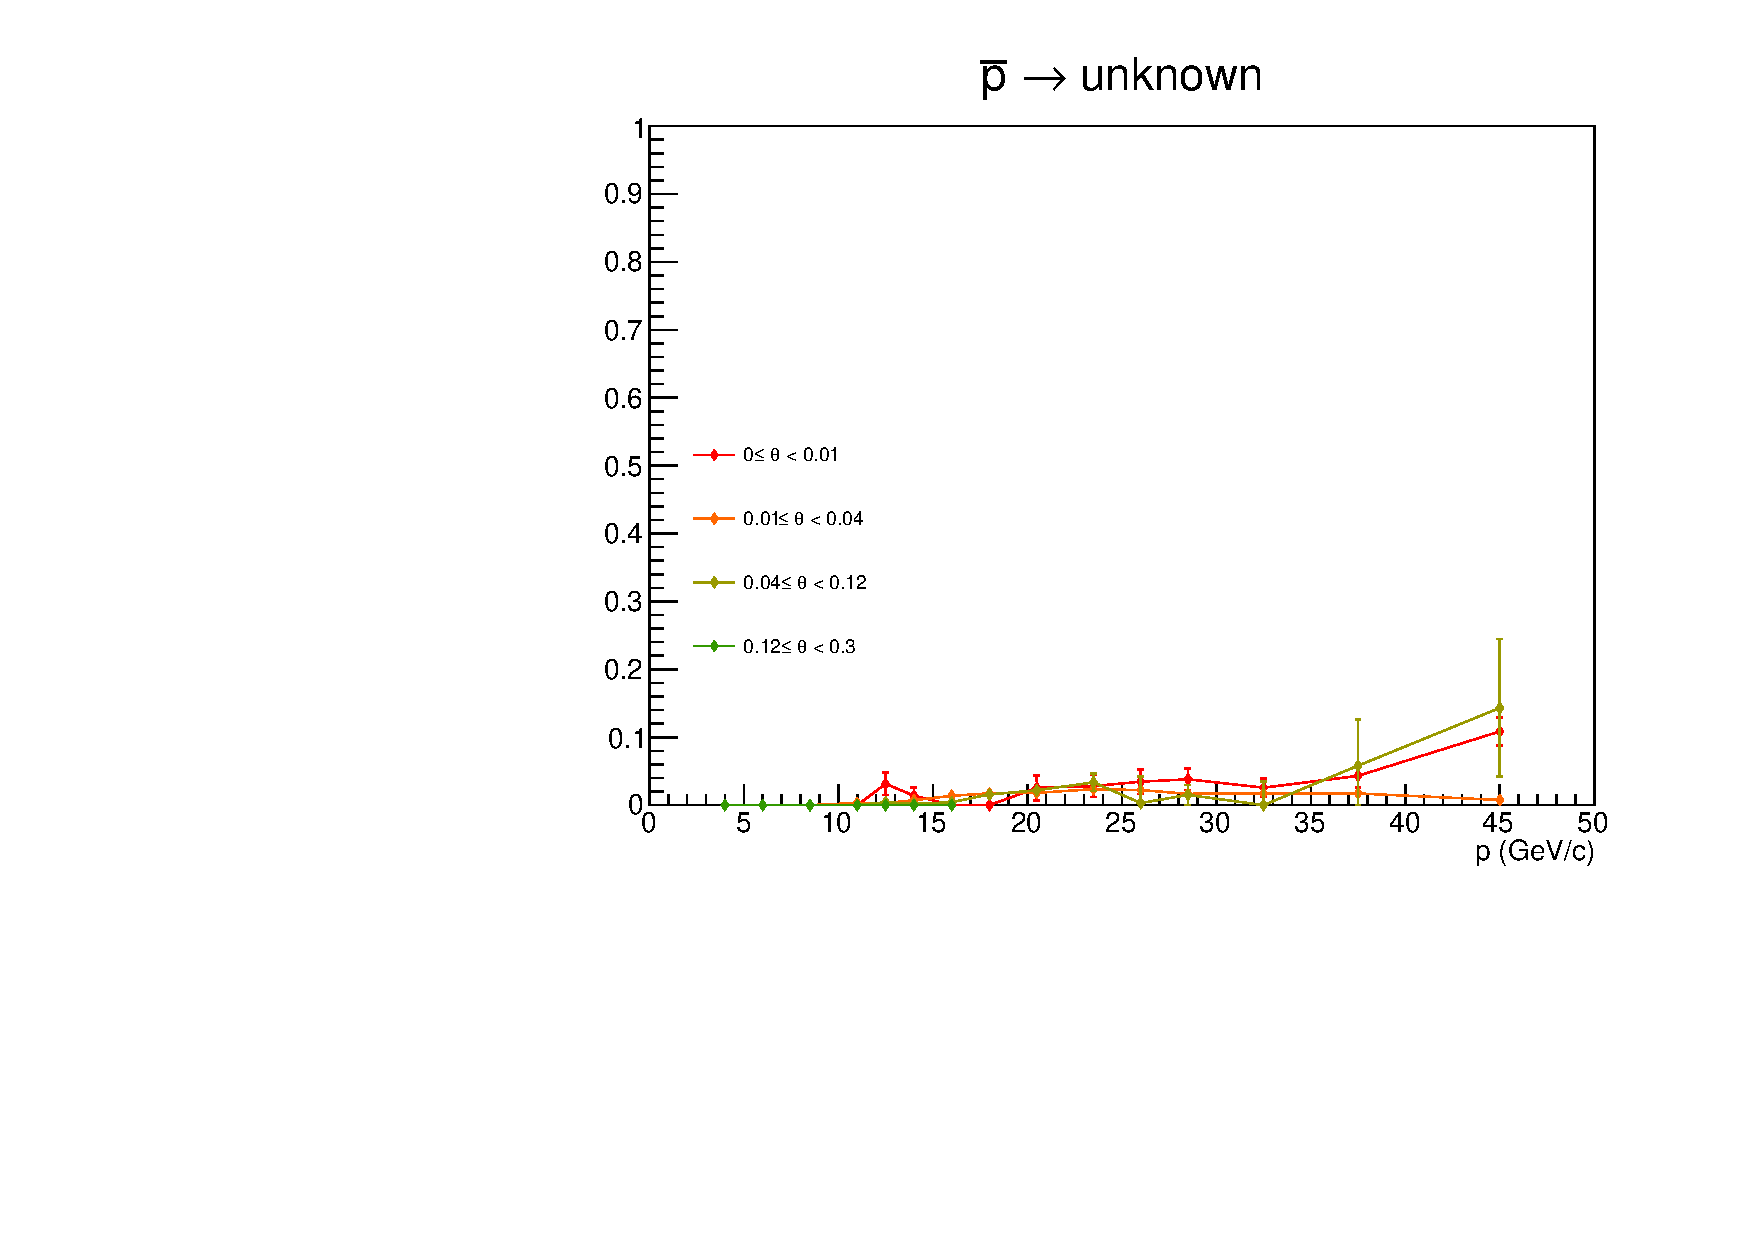
\includegraphics[scale=0.38]{./gfx/pm_u.pdf}
	\caption{Identification probabilities $\epsilon(p \rightarrow j)$ for $\bar{p}$.}
	\label{pic:Effpim}
\end{figure}

\newpage

\section{Problem at high $z$}

At some point it was discovered that in a particular kinematic region (35 GeV < $p_h$ < 40 GeV, $z$ > 0.7), non-linearities exist between the likelihood values of kaons and pions (Fig. \ref{pic:NonLin}). Instead of the expected separation between pions and kaons at $LH_{\pi} = LH_K$, pions are found at $LH_{\pi} < LH_K$.

\begin{figure}[!h]
  \centering
	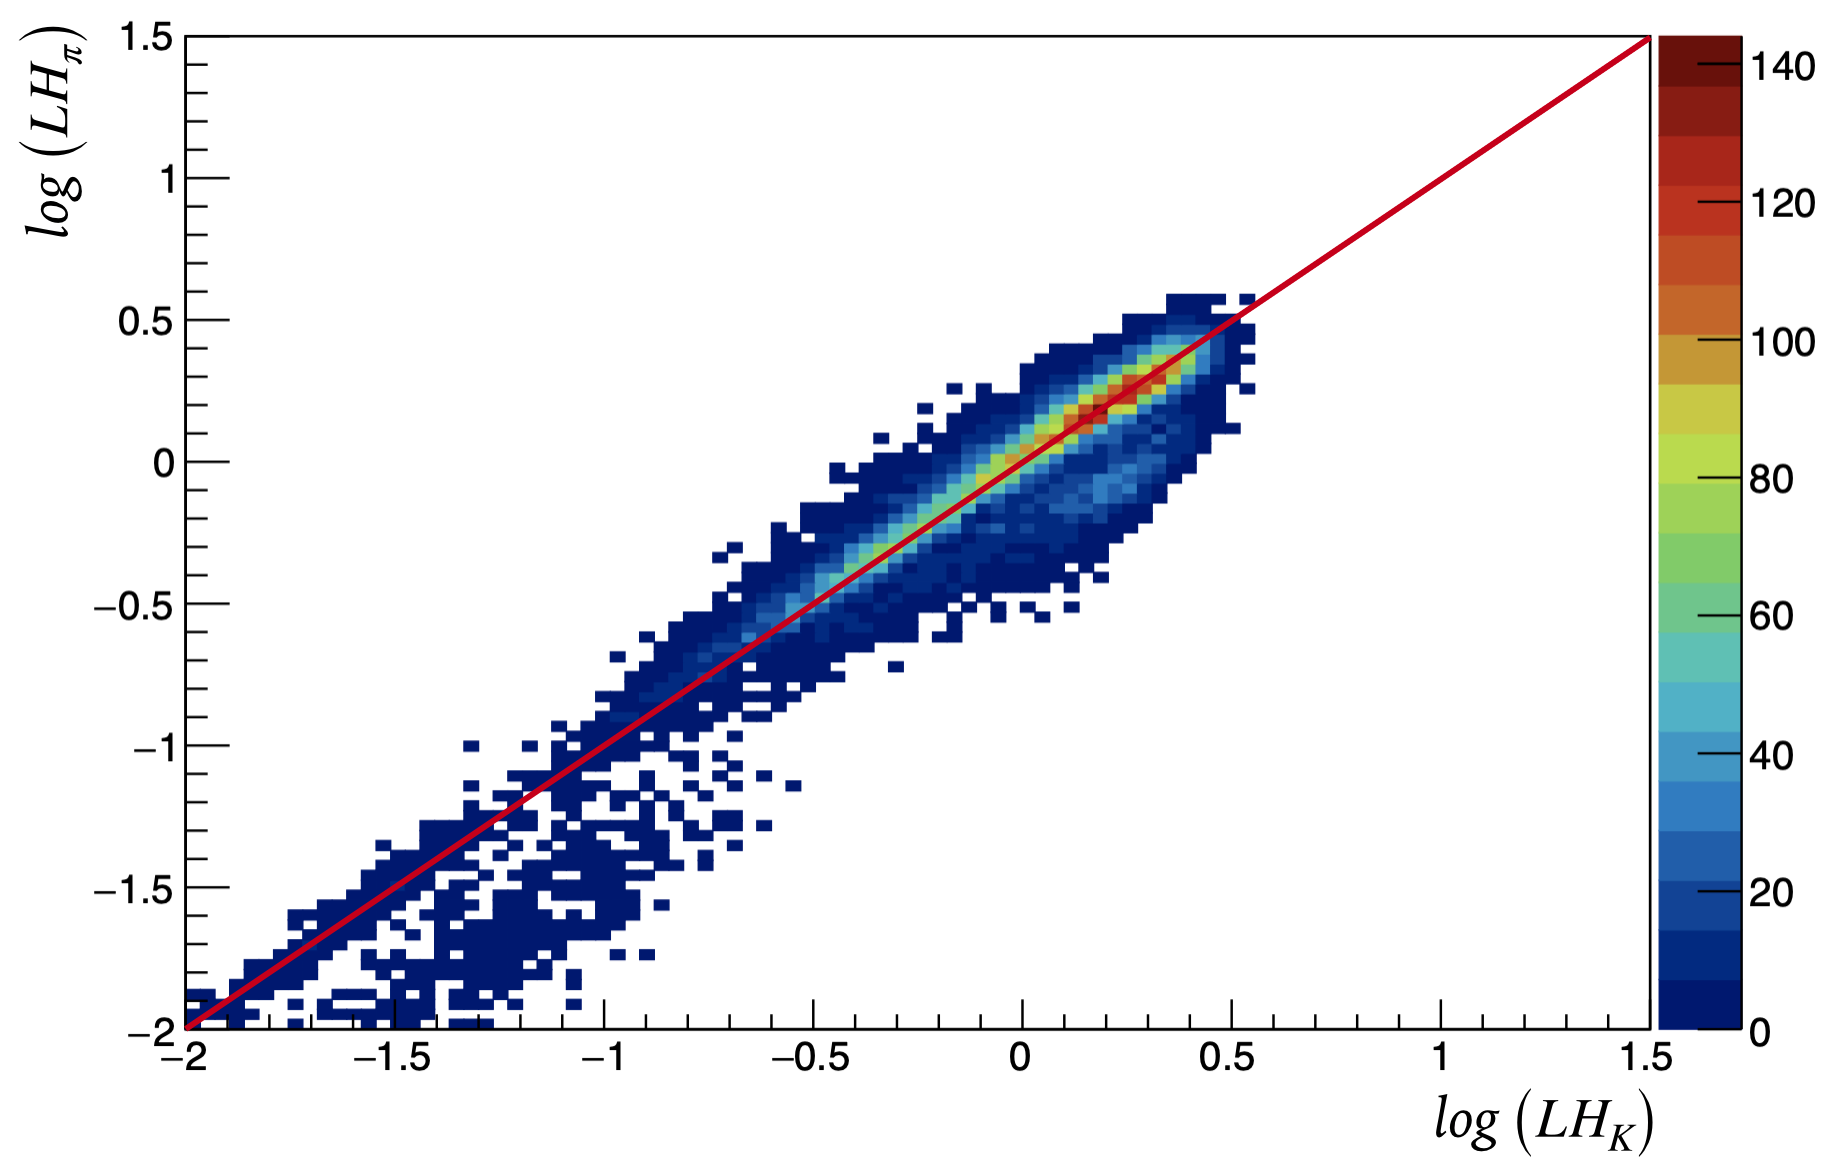
\includegraphics[scale=0.35]{./gfx/RICHLH.png}
	\caption{Likelihood for pions as a function of the likelihood for kaons using 2016 data.}
	\label{pic:NonLin}
\end{figure}

The larger the likelihood values are, the larger the effect is. This behaviour was already seen in 2006, 2007 and 2011 data (Fig. \ref{pic:NonLinother}). It was shown that the probability for the misidentification of pions as kaons differs from the value given in the RICH tables in this kinematic region using the $p_T$ spectra \cite{Marcin}. In order to see if the non-linearities are taken correctly into account in the RICH tables, the likelihood values for pions and kaonsare compared using the $K^0$ sample for high momenta and high $z$. This comparison is shown in Fig. \ref{pic:K0sample}, highlighting the fact that the problematic region is not covered by the $K^0$ sample and therefore the RICH table are not valid in this kinematic region. A new sample is then necessary for pions and it is obtained by using the $\rho^0$ decay into two pions. This sample contains, contrary to the $K^0$ one, events at high momenta and high $z$, which cover our region of interest. Moreover this sample shows the same symptoms as the SIDIS one (Fig. \ref{rho0}).

\begin{figure}[!h]
  \centering
	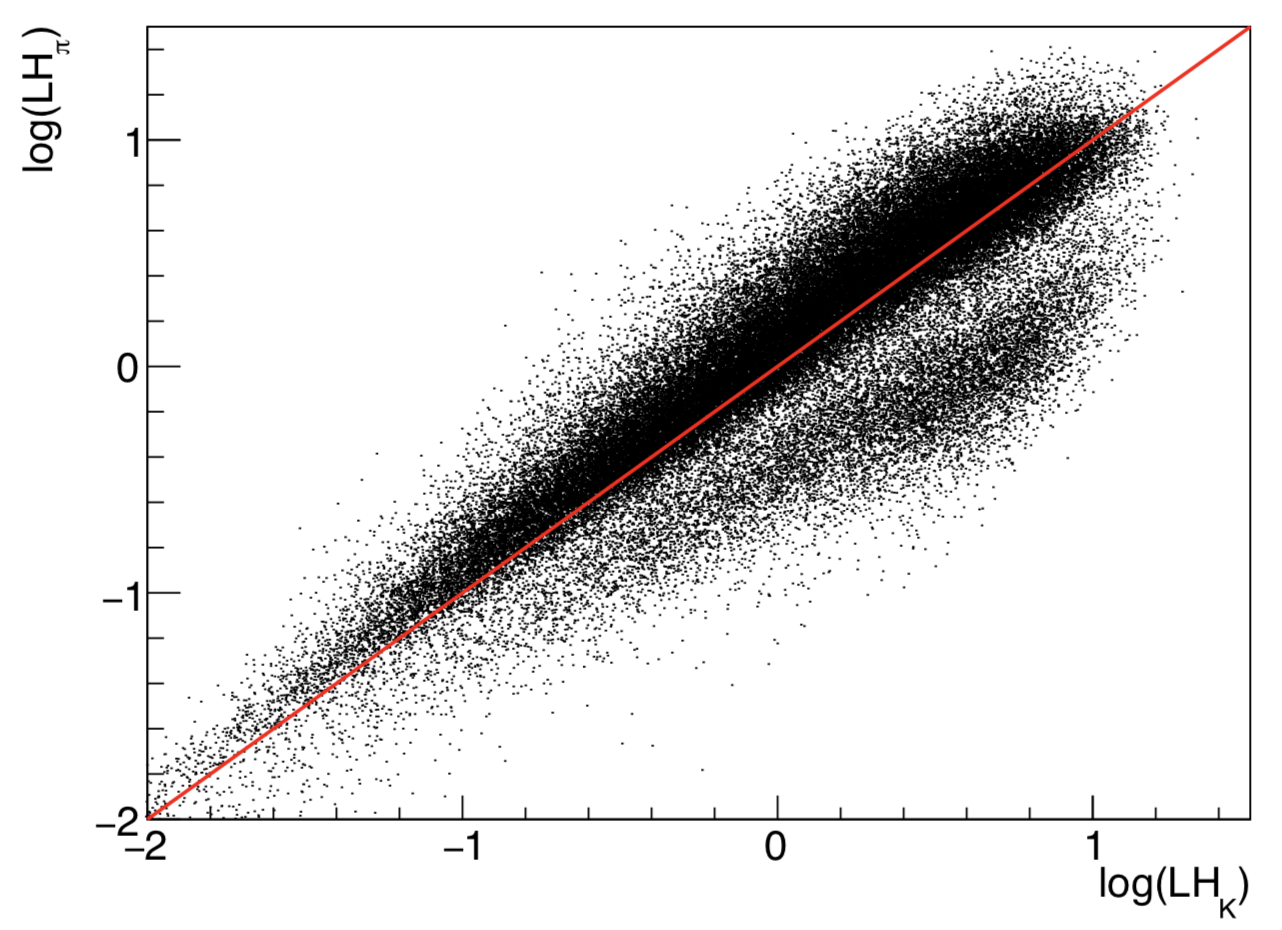
\includegraphics[scale=0.2]{./gfx/RICHLH2006.png}
  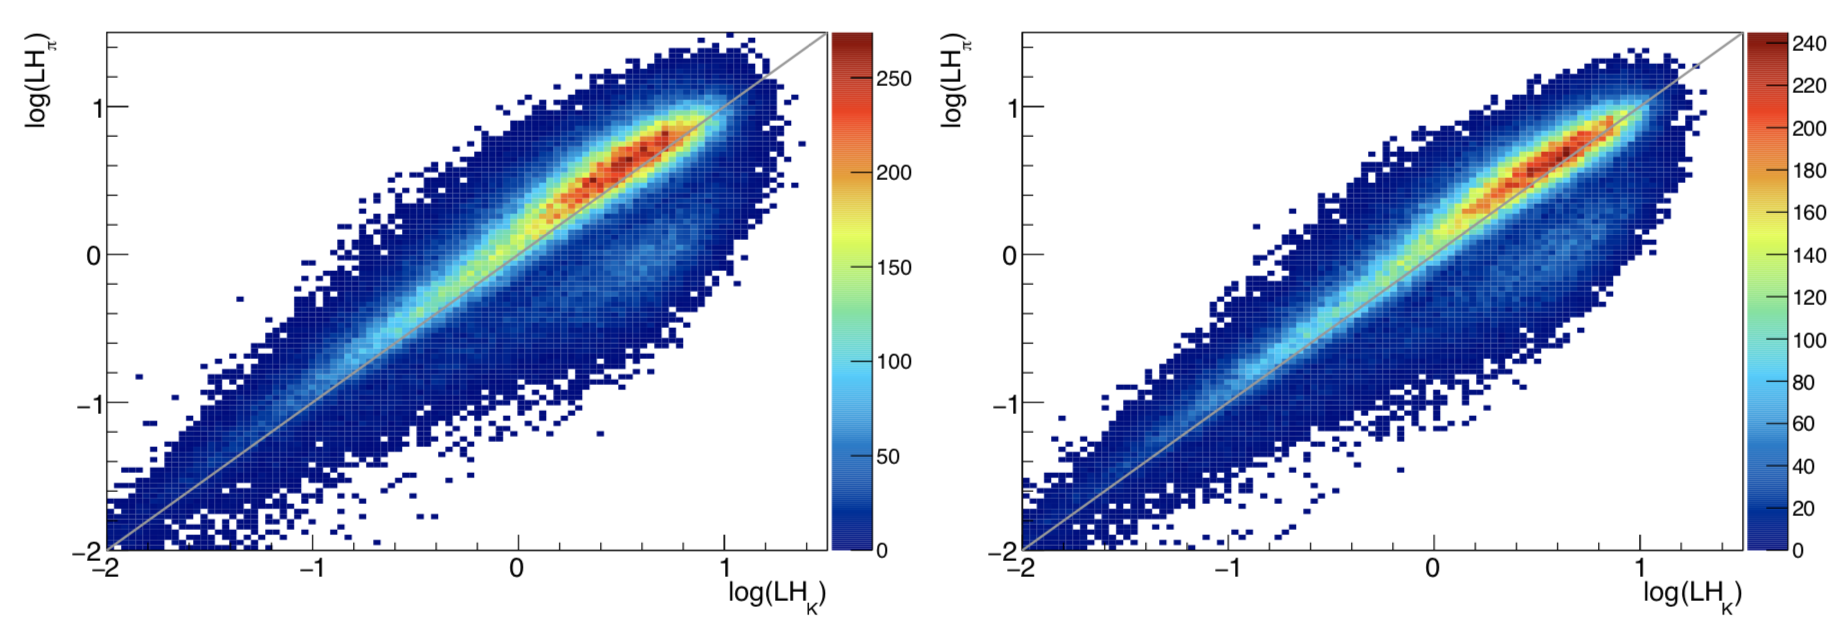
\includegraphics[scale=0.3]{./gfx/RICHLH2011.png}
	\caption{Likelihood for pions as a function of the likelihood for kaons using (from left to right) 2006, 2007 and 2011 data.}
	\label{pic:NonLinother}
\end{figure}

\section{PID using $\rho^0$}

In order to calculate the RICH tables at high momenta and high $z$, a sample of $\rho^0$ candidates decaying into two charged pions is used. The selection is described in the following.

\subsection{Data Selection}

The $\rho^0$ meson decay length is too short to separate the primary and the decay vertices. Therefore all outgoing particles from a primary vertex are taken into account for the search of possible $\rho^0$ mesons. This results in a large combinatorial background like in the case of the $\Phi$ mesons. The branching ratio of the decay into two pions is $\sim$ 100\%.

\begin{enumerate}
  \item Selection of possible good events with $\rho^0$ mesons
  \begin{itemize}
    \item At least 3 outgoing particles including scattered muon
    \item Loop over all outgoing particles
    \item Oppositely charged pairs of hadrons (none is a muon)
  \end{itemize}
  \item Select good hadron tracks
  \begin{itemize}
    \item First measured position in front of SM1
    \item Last measured position behind SM1
    \item Skip possible muon candidates with last measured positions $>$ 3300 cm or $X/X_0$ $>$ 10
    \item Transverse momentum with respect to the mother particle larger than 23 MeV to suppress electrons
    \item Good reconstructed track with $\chi^2$/ndf $<$ 10
  \end{itemize}
  \item Additional cuts
  \begin{itemize}
    \item $p_h$ $>$ 1 GeV/$c$
    \item Mass difference smaller than 250 MeV/$c^2$ between the $\rho^0$ mass and the invariant mass of the two decay hadrons assuming the pion masse.
    \item Invariant mass of the two hadrons smaller than 1.04 MeV/$c^2$ assuming the kaon mass to supress $\Phi$ mesons.
  \end{itemize}
\end{enumerate}

The selection steps are similar to the selection of the $\Phi$ candidates. In the first step, primary vertices with oppositely charged hadron pairs are selected. During the second selection step, only particles with a measured momentum are kept and possible electrons are removed with a cut on low transverse momentum. In addition possible muon candidates are removed. Similar to the selection of $\Phi$ meson candidates, a large combinatorial background is obtained.

\subsection{Fit and results}


\section{Comparison of the efficiencies of 2006 to 2016}
